\section{Émbolos} \label{s:section_01}

Para comenzar la elaboración del informe correspondiente a la parte de arquitectura de los motores alternativos, cabe estudiar en primer lugar la morfología y funcionamiento de los émbolos, elementos claves en los motores de alternativos; ya que estos constituyen la frontera móvil de la cámara de combustión. La superficie del émbolo será un aspecto importante a considerar, pues deberá tener la morfología adecuada para conseguir una buena turbulencia y un correcto mezclado combustible-aire.\\

Se estudiarán y comentarán tanto los émbolos de ciclo Otto como los de Diesel, así como otros elementos importantes como bielas, bulones o segmentos, y se irán abordando las distintas cuestiones planteadas durante la realización de la práctica. Así, la figura \ref{fig:emb_comp} muestra un esquema del conjunto con todos los elementos previamente mencionados, a falta de su acople en el cigüeñal.

\begin{figure}[H]
	\centering
	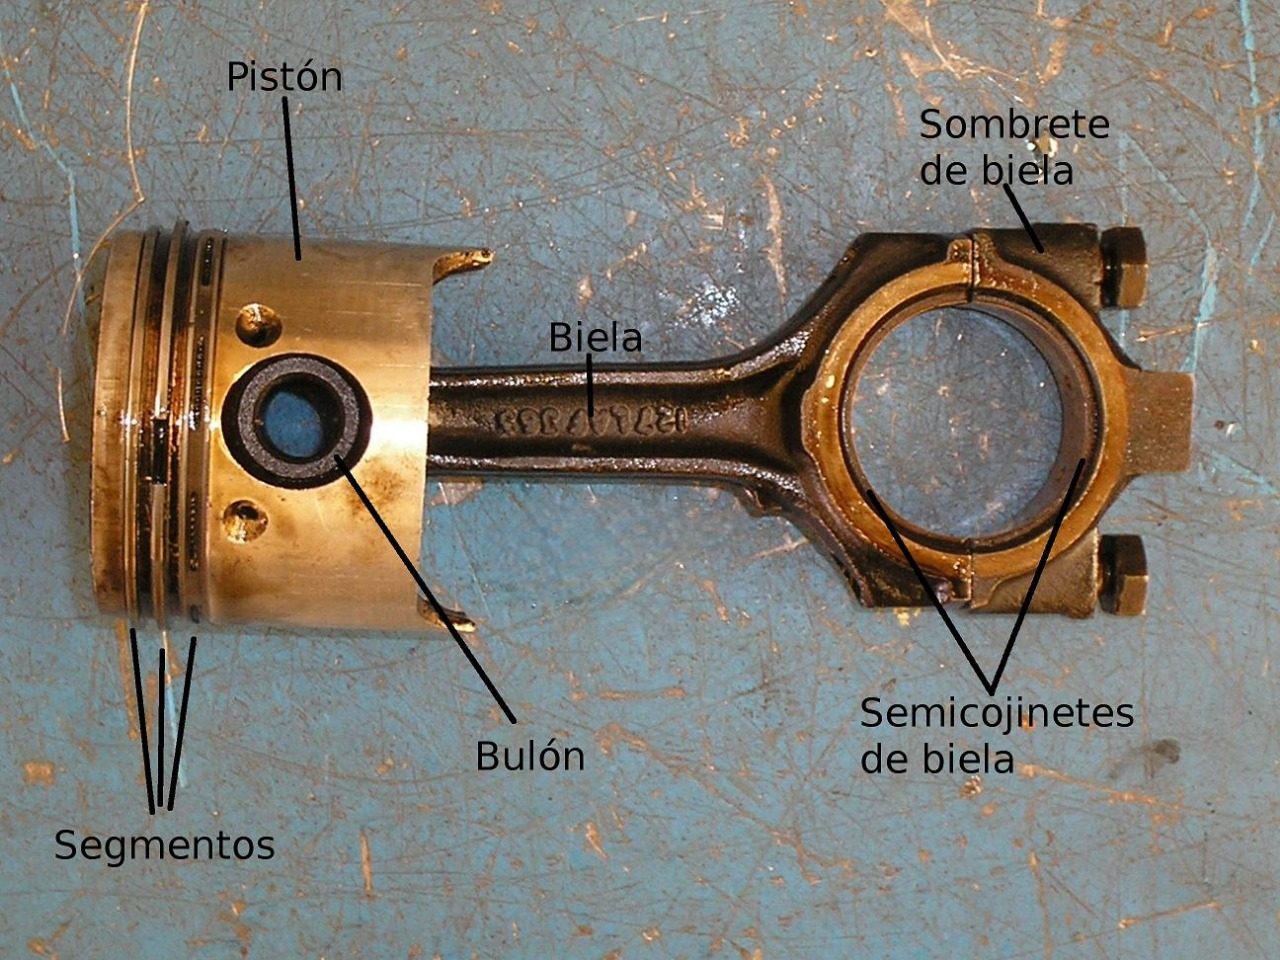
\includegraphics[width=0.6\linewidth]{Figures/01/m1/componentes.jpg}
	\caption{Conjunto de los distintos componentes a montar en el cigüeñal.}
	\label{fig:emb_comp}
\end{figure}

\subsection{Émbolos} \label{ss:piston}

En primer lugar se van a analizar las diferencias que existen entre los émbolos de los motores Otto y Diesel. Por un lado, los émbolos en motores Otto suelen operar a presiones y temperaturas más bajas que los motores Diesel y, por tanto, estos primeros serán más ligeros y pequeños. Por otro lado, los émbolos de los motores Diesel presentarán una mayor resistencia y robustez debido a lo anteriormente mencionado.\\

Debido a estas condiciones y solicitaciones estructurales, será de vital importancia la correcta elección de los materiales que los conforman. Los émbolos de ciclo Otto se fabrican fundamentalmente de aluminio, lo que les otorga esa ligereza característica. Por su parte, los émbolos de ciclo Diesel son más robustos y pesados, pues se fabrican principalmente de aleaciones pesadas como aceros forjados o hierro fundido. Como se ha comentado anteriormente, la diferencia entre ambos es que los Diesel tienen que soportar temperaturas y presiones más altas que los Otto, de ahí que estos últimos puedan emplear aleaciones ligeras de aluminio, lo que les confiere mayor conductividad térmica y capacidad para trabajar a muy altas revoluciones.\\

En cuanto al diseño de la geometría del émbolo está influenciado por los fenómenos de dilatación que sufren las diferentes zonas del émbolo. Como este fenómeno va disminuyendo a lo largo del émbolo (al ir disminuyendo la temperatura), este tendrá una forma troncocónica para compensar la dilatación en las diferentes zonas del material. De esta manera se consigue reducir el desgaste por fricción con las paredes. Esto se aprecia en la figura \ref{fig:emb_croq}, donde se puede observar un croquis de la cabeza del émbolo, y sus distintas dimensiones en la cabeza y en las partes superior e inferior de la falda. Estas medidas han sido tomadas durante la práctica de laboratorio.

\begin{figure}[H]
	\centering
	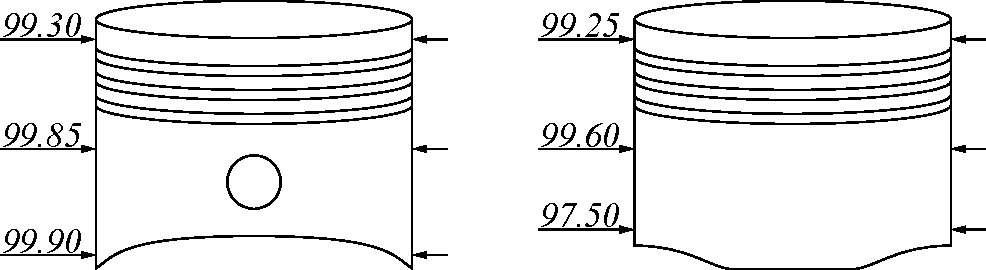
\includegraphics[width=0.6\linewidth]{Figures/01/m1/croq_3.pdf}
	\caption{Croquis del émbolo con las distintas medidas en la cabeza y partes superior e inferior de la falda.}
	\label{fig:emb_croq}
\end{figure}

Otros aspecto a analizar son las cavidades practicadas en las cabezas de los émbolos. Los motores Diesel presentan estas oquedades con el objetivo de facilitar la atomización y mezcla del combustible con el aire. Esto se puede ver en la figura \ref{fig:emb_diesel} donde la forma y el tamaño de la oquedad favorecen una mejor mezcla del combustible.

\begin{figure}[H]
	\centering
	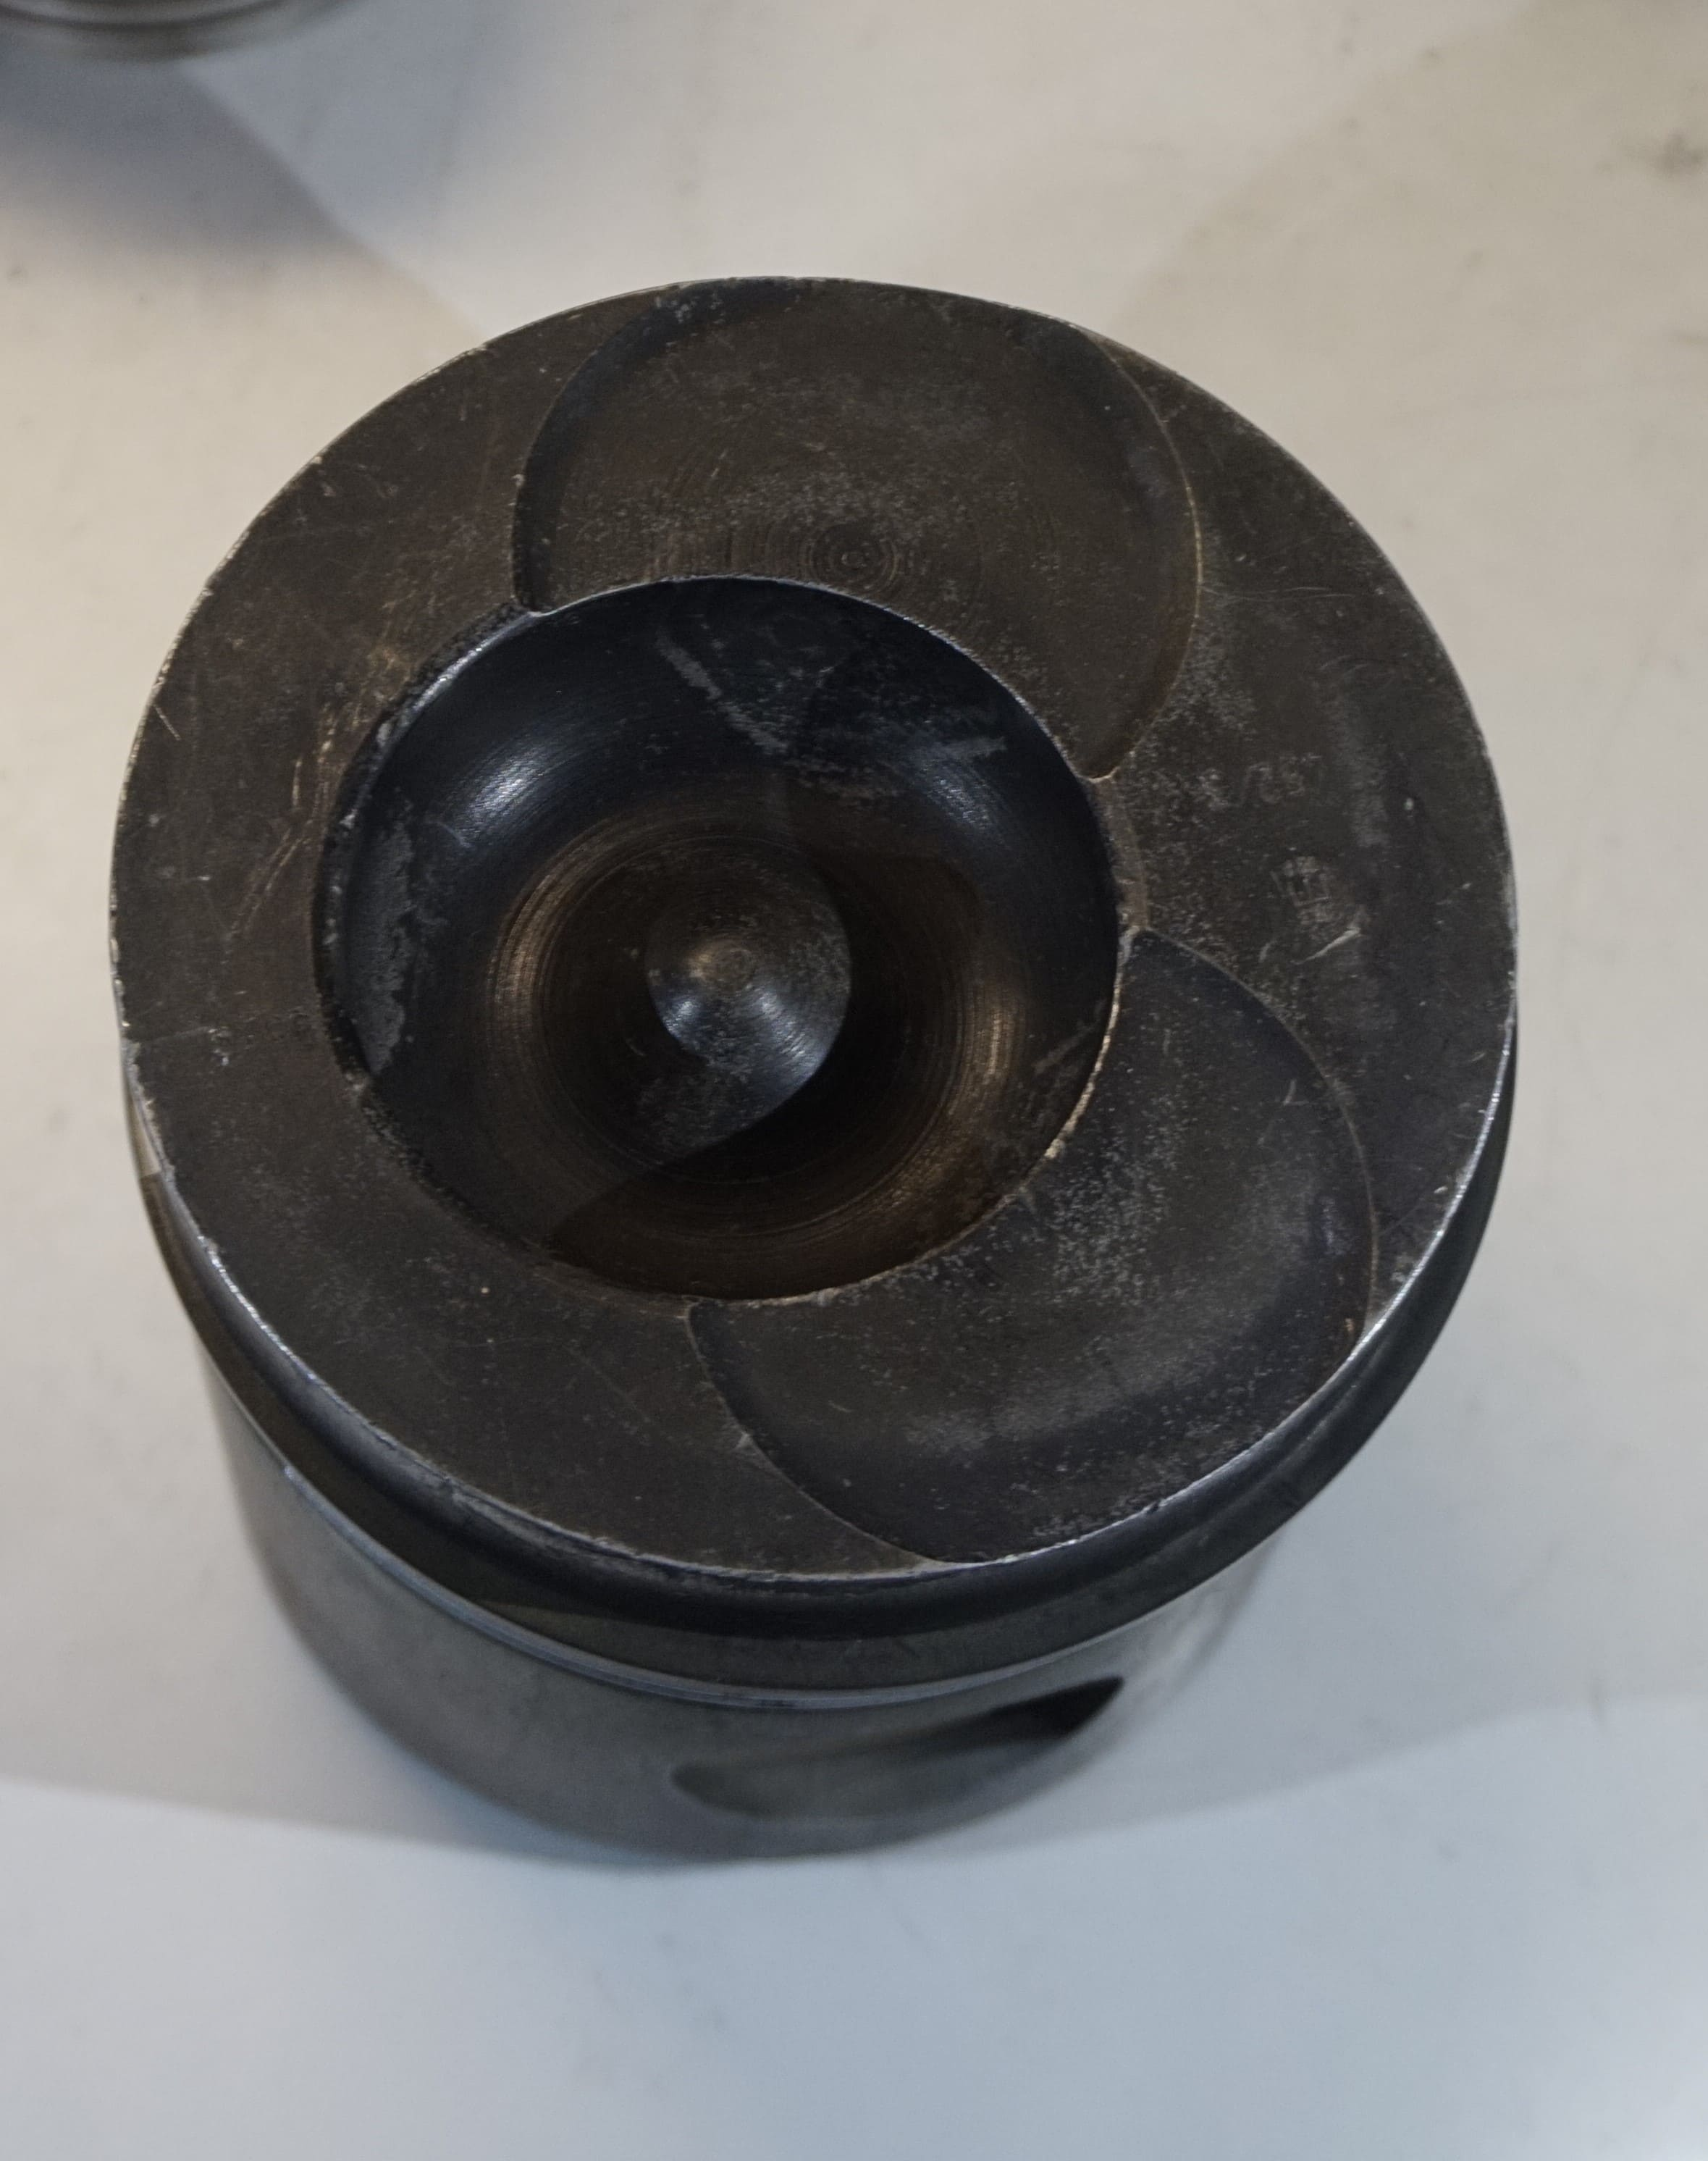
\includegraphics[width=0.275\linewidth]{Figures/01/m1/cil_diesel.jpg}
	\caption{Émbolo de motor Diesel.}
	\label{fig:emb_diesel}
\end{figure}

Por otro lado, los émbolos de los motores Otto presentan unas superficies más planas que las Diesel, como se ha comentado anteriormente. Sin embargo, estos también presentan ciertos rebajes como se puede ver en la figura \ref{fig:emb_gas}, sirviendo estas principalmente para mejorar el mezclado de aire y combustible o, como es el caso de la de la figura \ref{fig:emb_gas_2}, para evitar el contacto entre válvula y émbolo.

\begin{figure}[H]
	\centering
	\begin{subfigure}[b]{0.45\textwidth}
		\centering
		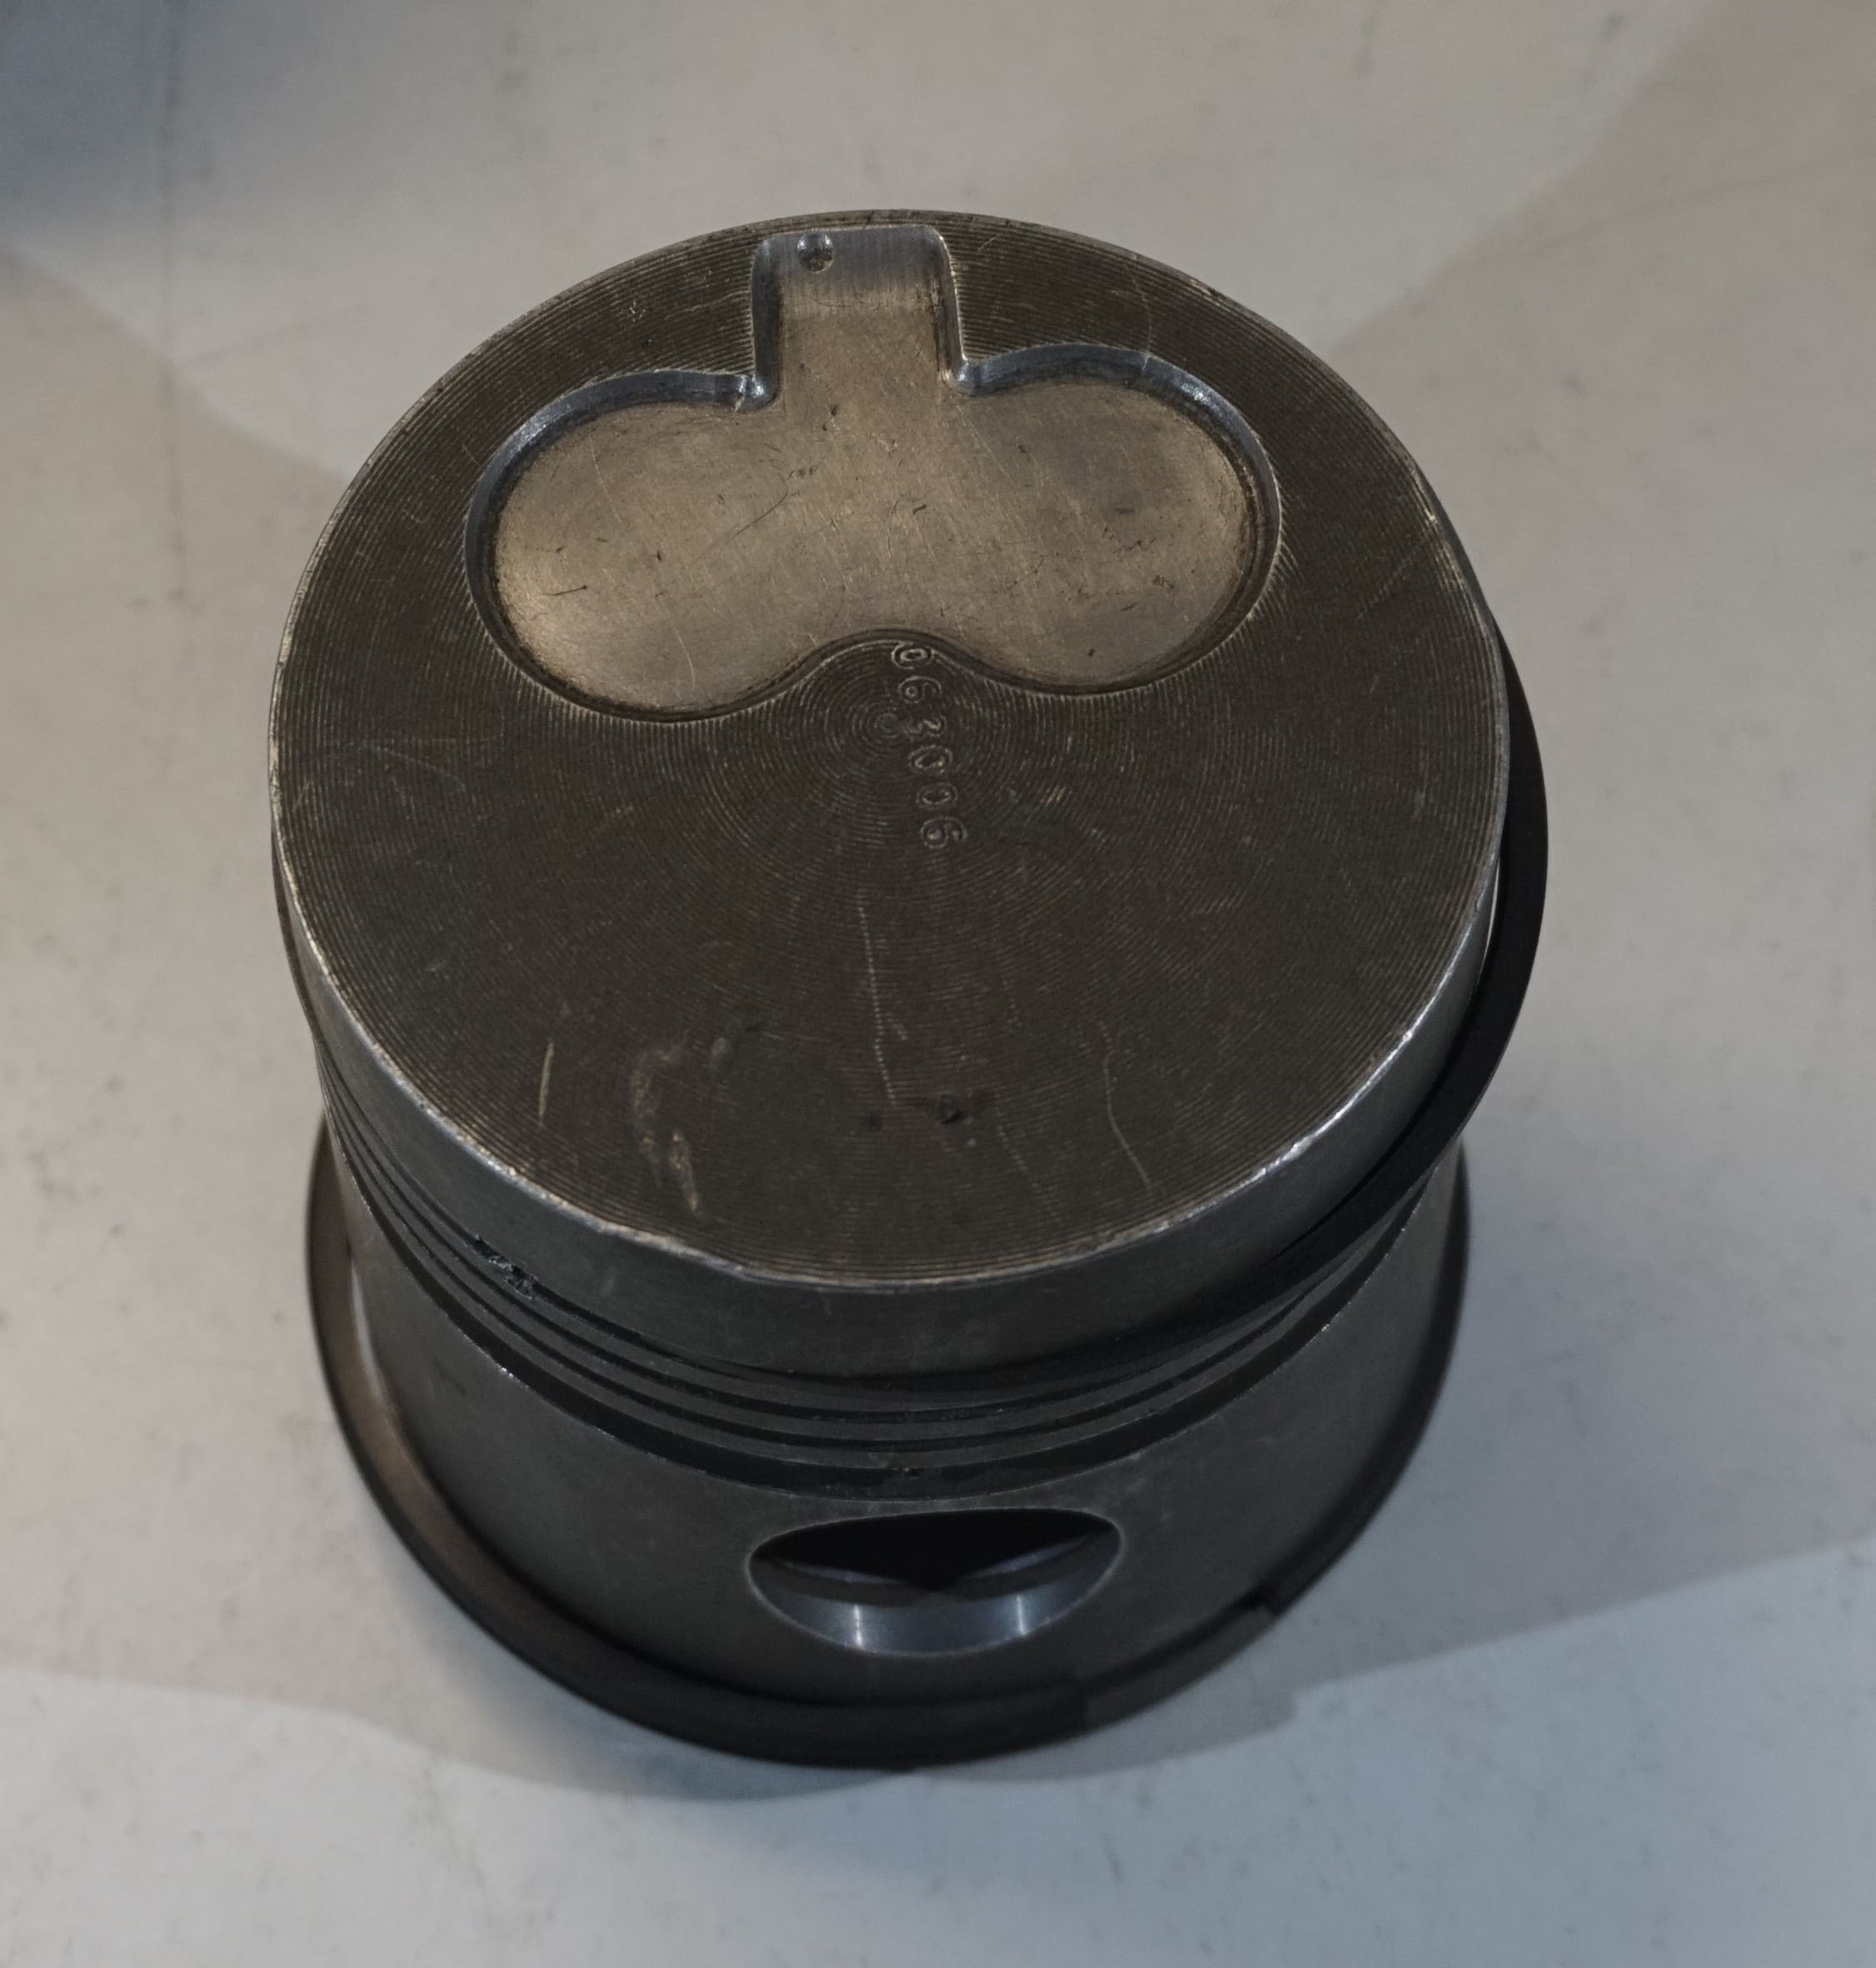
\includegraphics[width=\linewidth]{Figures/01/m1/cil_gas_1.jpg}
		\caption{Émbolo con rebaje para mezcla.}
		\label{fig:emb_gas_1}
	\end{subfigure}
	\hfill
	\begin{subfigure}[b]{0.45\textwidth}
 		\centering
 		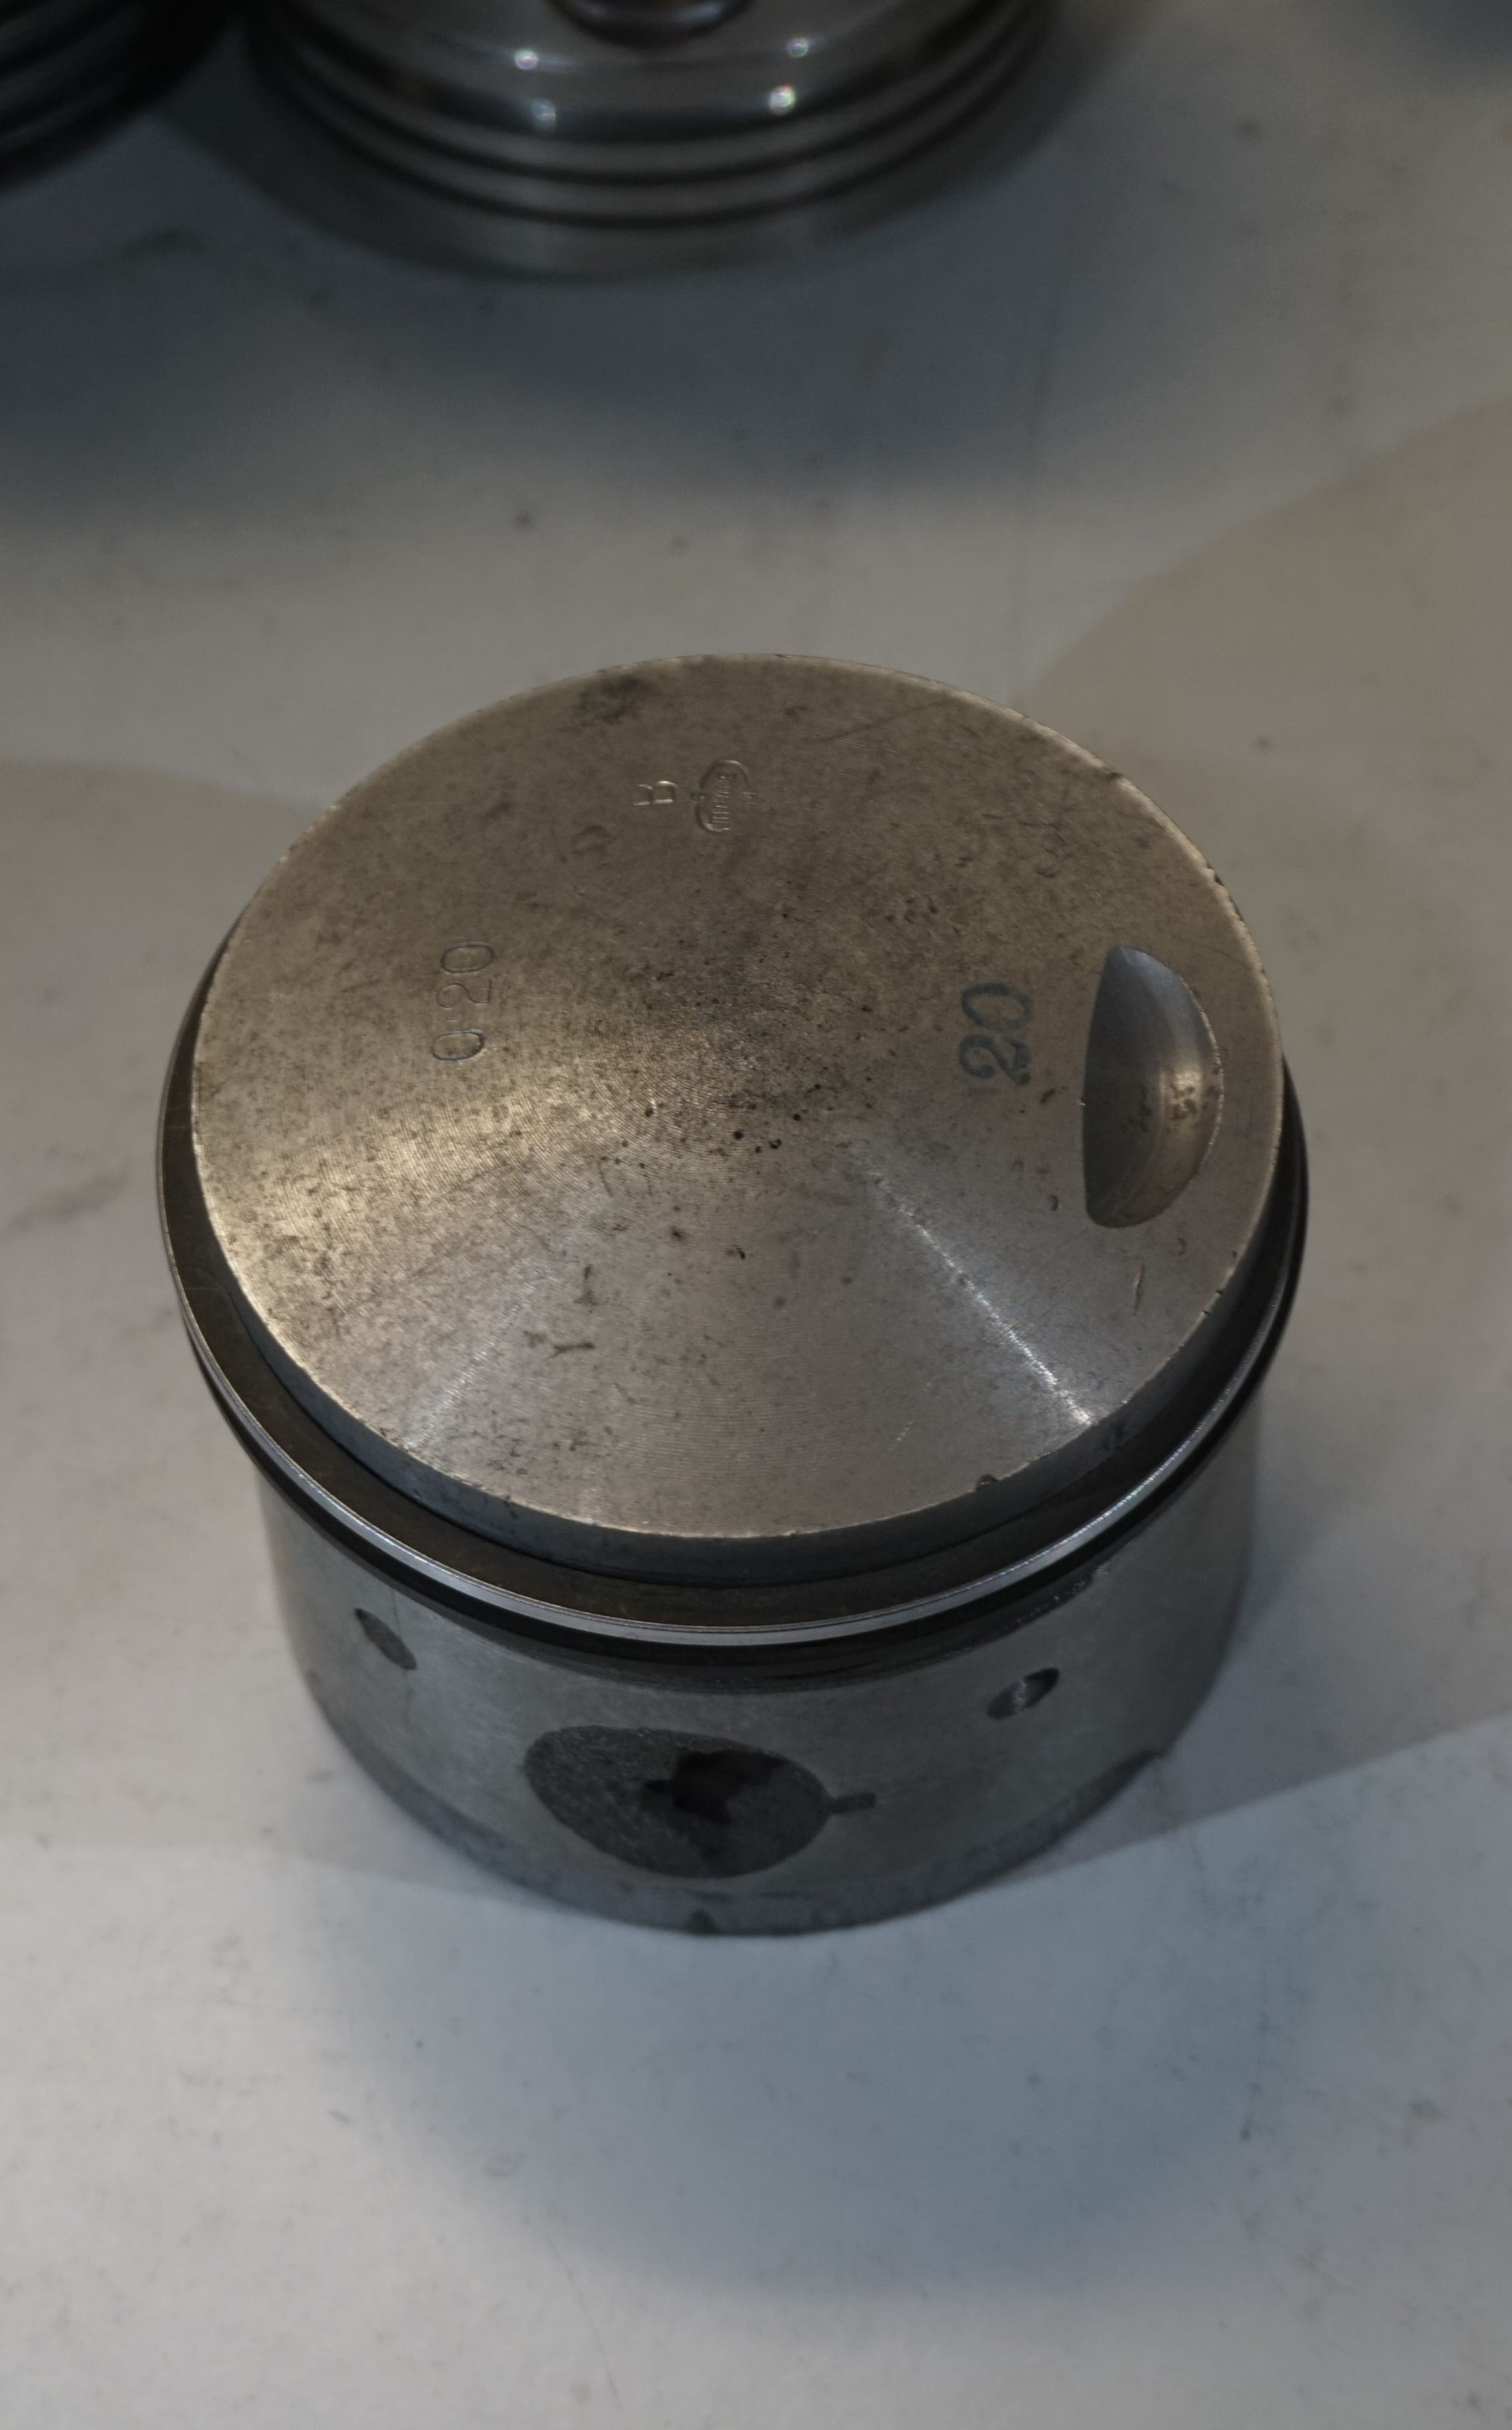
\includegraphics[width=\linewidth]{Figures/01/m1/cil_gas_2.jpg}
 		\caption{Émbolo con rebaje para evitar contacto.}
		\label{fig:emb_gas_2}
	\end{subfigure}    
	\caption{Émbolos de motor Otto.}
	\label{fig:emb_gas}
\end{figure}


Finalmente, se va a analizar el espesor del émbolo, otro aspecto crucial para resistir las elevadas presiones y temperaturas de la cámara de combustión. Un espesor demasiado pequeño podría ocasionar graves problemas de resistencia y deformación, además de deficiencias de disipación y transmisión de calor, dando lugar a puntos calientes. Por otro lado, un espesor demasiado elevado podría incurrir en problemas de pesos elevados, incrementando significativamente las fuerzas inerciales del motor, empeorando su comportamiento a altos ciclos y acelerando su desgaste.

\subsection{Bulones y bielas} \label{ss:wristpins}

Para proseguir, se van a estudiar otros elementos claves en los motores de combustión tales como los bulones y las bielas (si bien estas se comentarán con mayor detalle en la sección \ref{ss:conrod}). Estos componentes serán los encargados de unir y transmitir el movimiento generado por el émbolo al cigüeñal. Así, tras haber analizado el material de construcción de los émbolos, cabe destacar también las aleaciones empleadas en bulones. Los bulones son los componentes que unen el émbolo con la biela, de forma que el movimiento del émbolo pueda ser transmitido desde este al cigüeñal mediante la unión bulón-biela. Dado que el bulón atraviesa el émbolo en dirección transversal a su eje, y se acopla en su punto medio a la biela, paralela al eje del émbolo, los esfuerzos que deberá soportar principalmente el bulón serán esfuerzos de flexión. Además, deben tener gran resistencia a fatiga para soportar los ciclos del motor. Por ello, se fabricarán fundamentalmente de aceros de alta resistencia y con tratamientos térmicos que le confieran las propiedades necesarias para soportar los estados de carga previamente mencionados.

\subsection{Segmentos} \label{ss:pistonrings}

Para finalizar, los segmentos son esos “anillos” que se colocan en las ranuras de la cabeza del pistón y se encargan de sellar el espacio entre el émbolo y el cilindro , para evitar el escape de los gases y mantener una correcta lubricación. Por ello, deberán soportar altas temperaturas, fricción y desgaste, lo que hace idónea la utilización de aleaciones de hierro fundido o acero, además de incorporar tratamientos y recubrimientos para aumentar su vida útil.\\

No todos los segmentos son iguales, como se aprecia en la figura \ref{fig:emb_side}. Los segmentos de fuego y compresión (superiores) están diseñados para soportar elevadas temperaturas y presiones (al estar más cerca de la cámara de combustión), con el objetivo de realizar un sellado eficaz en la cámara de combustión y evitar el escape de los gases. Por otro lado, los segmentos rascadores (inferiores) tienen la función de controlar la cantidad de aceite, retirando el exceso de este para evitar que llegue a la cámara de combustión y evitando que se queme una mayor cantidad de aceite de la prevista. Además, aseguran la correcta limpieza de las paredes y evitan la presencia de suciedad o residuos en estas. Es clave mantener los segmentos en buen estado y con las dimensiones correctas, para asegurar el sellado y prevenir fallos por desgaste. Todo esto asegurará un correcto funcionamiento del motor, y aumentará su vida útil.\\

\begin{figure}[H]
	\centering
	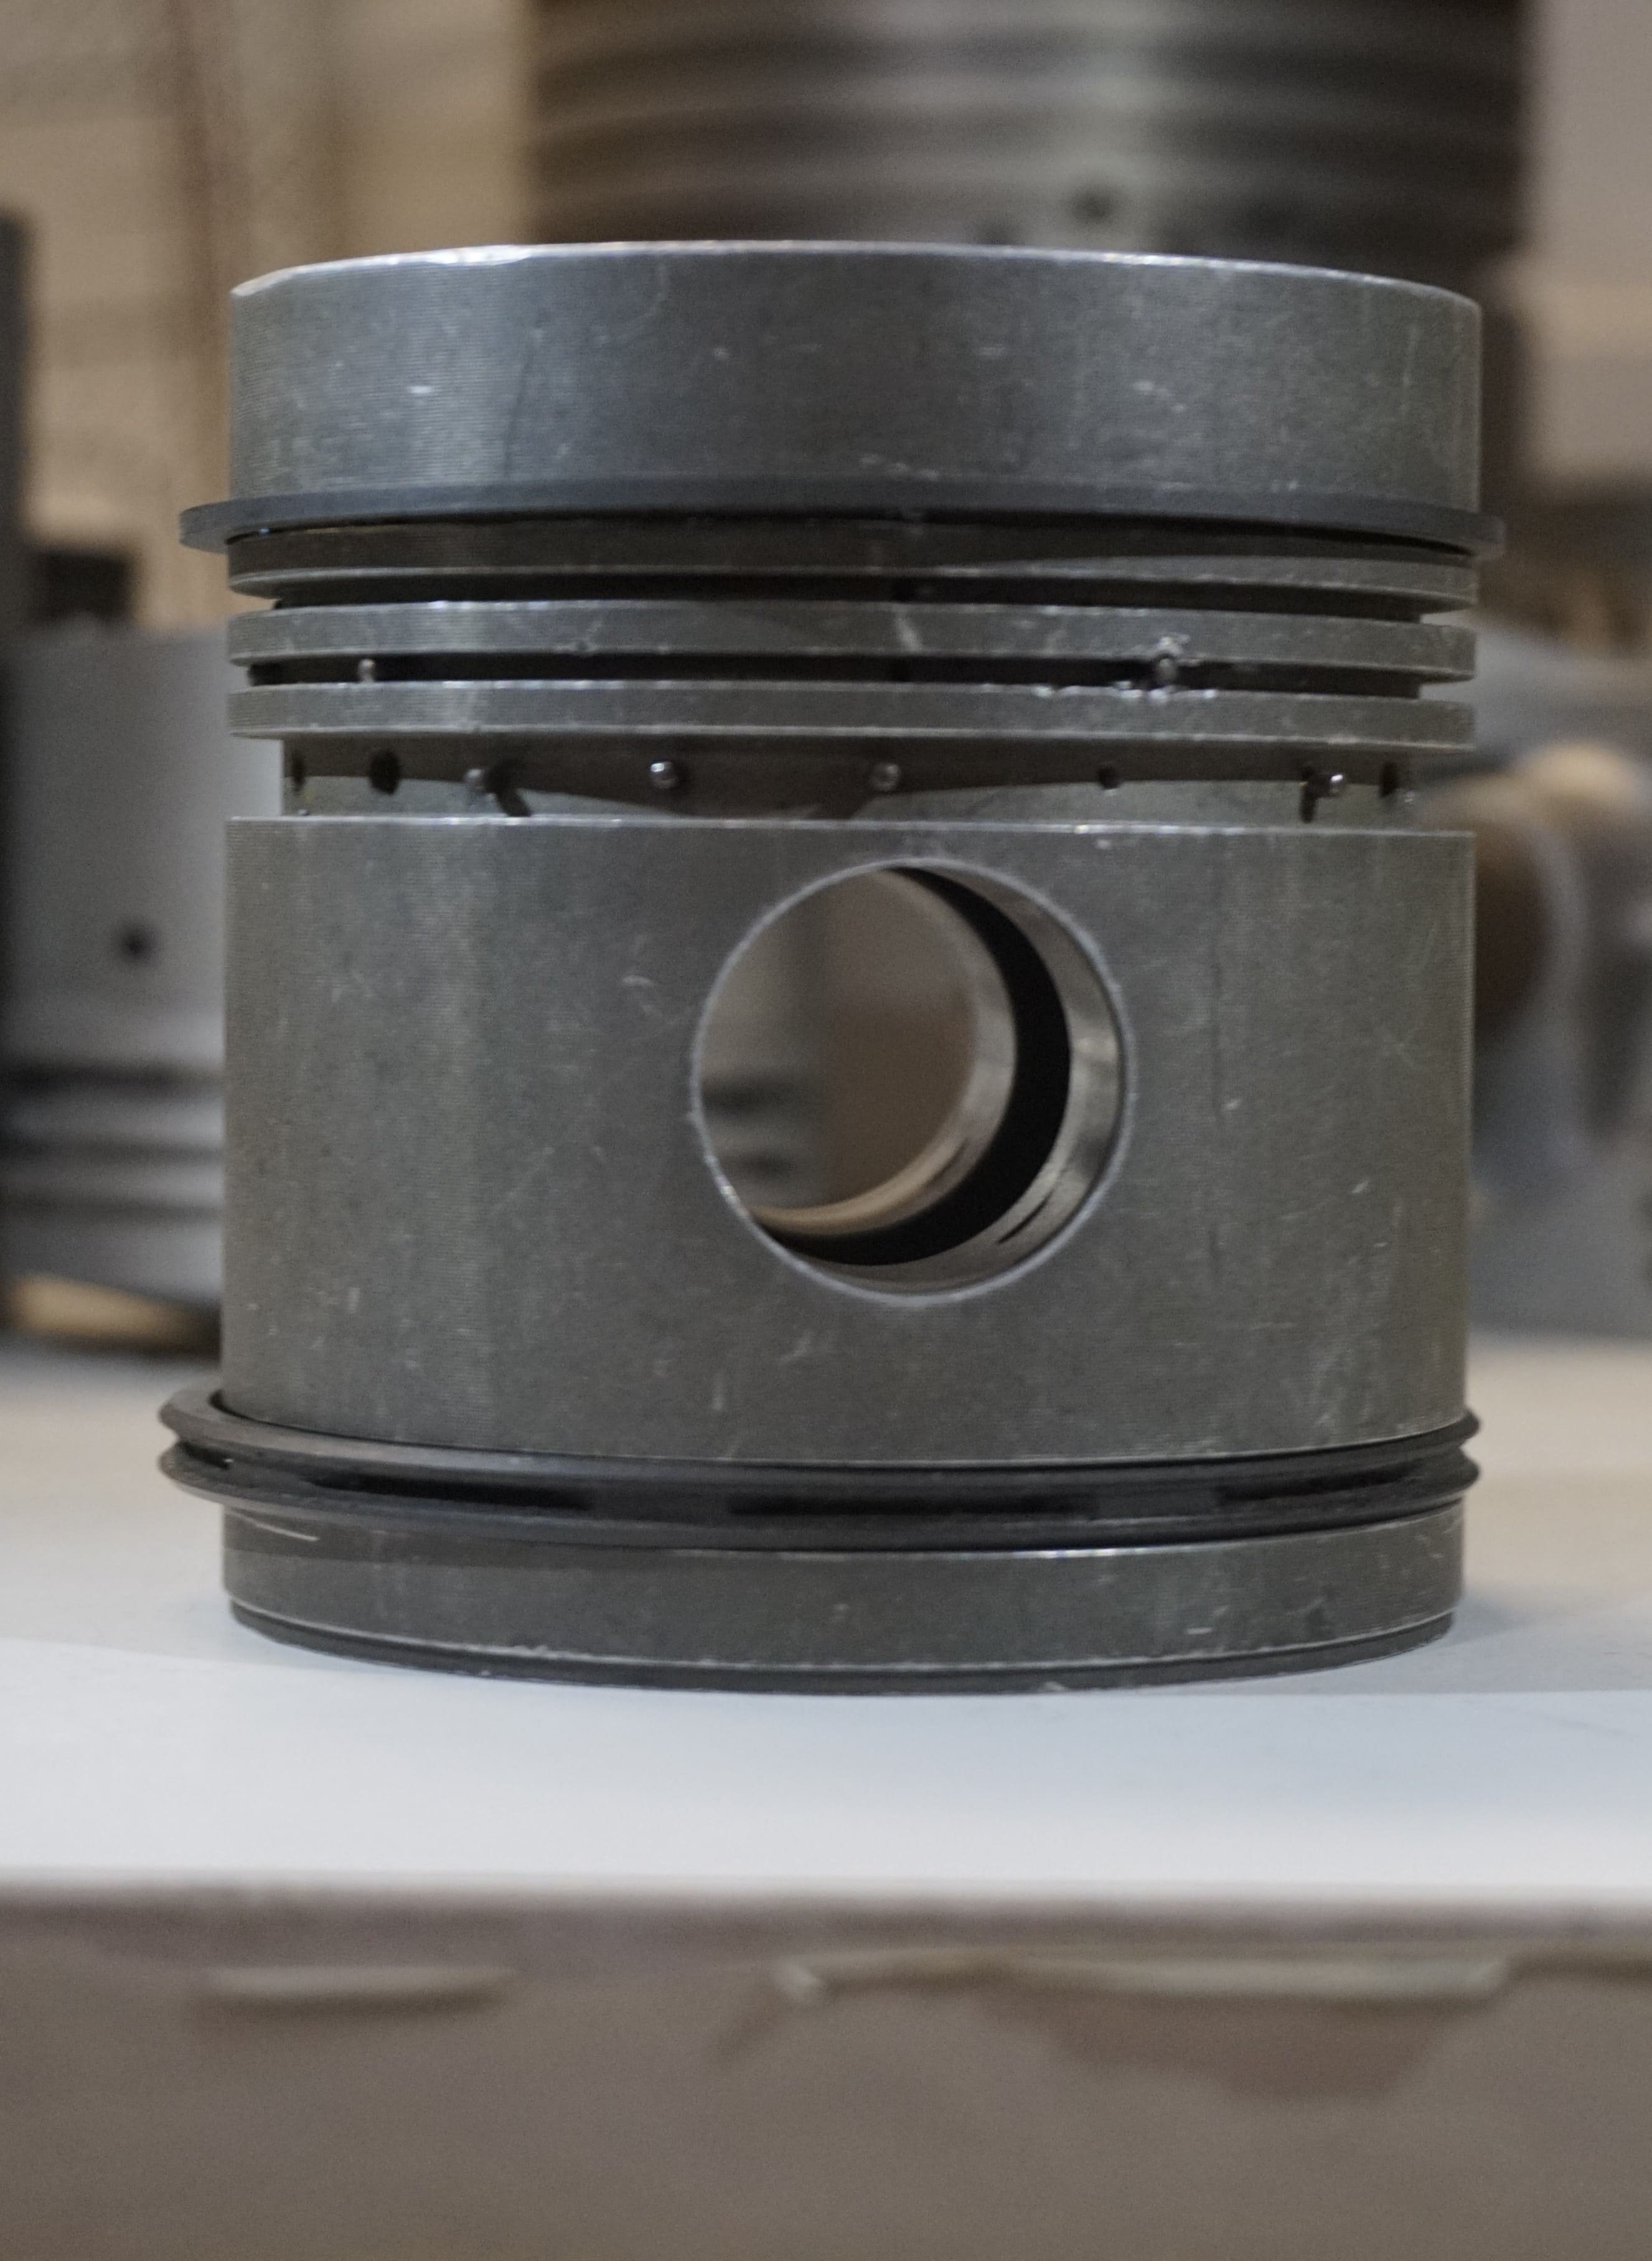
\includegraphics[width=0.5\linewidth]{Figures/01/m1/cil_side.jpg}
	\caption{Segmentos y agujero para el instalación del bulón.}
	\label{fig:emb_side}
\end{figure}

Estos segmentos deben ajustarse correctamente al pistón. Esto implica que estén correctamente asentados en las ranuras, pero no excesivamente apretados. Esto se debe a que, por un lado, no deben tener holguras que puedan provocar excesivo movimiento y que se deslicen durante el funcionamiento del motor, pues podría afectar negativamente a su funcionamiento al no cumplir adecuadamente con su misión selladora. Por otra parte, si están demasiado apretados podría generarse demasiada fricción y con ello elevadas temperaturas, además de no permitir ningún tipo de dilatación térmica. Es por ello que los segmentos deben estar asentados firmemente en las correspondientes ranuras, asegurando su correcto sellado, pero permitiendo su ligera expansión durante el funcionamiento del motor. De esta forma la vida útil de estos componentes, y por consiguiente la del motor, será mayor.

\newpage

\section{Distribución} \label{s:section_02}

A continuación, se estudiará el mecanismo de distribución de un motor alternativo, siendo este un sistema fundamental en los motores de combustión interna dado que se encarga de controlar la apertura y cierre de las válvulas en sincronización con los pistones y el cigüeñal. Su función principal es la de permitir la entrada de la mezcla aire-combustible y la salida de los gases de escape. En esta mesa se analizarán las distintas piezas fundamentales y comunes en cualquier sistema de distribución, válvulas y árbol de levas.
\begin{figure}[H]
	\centering
	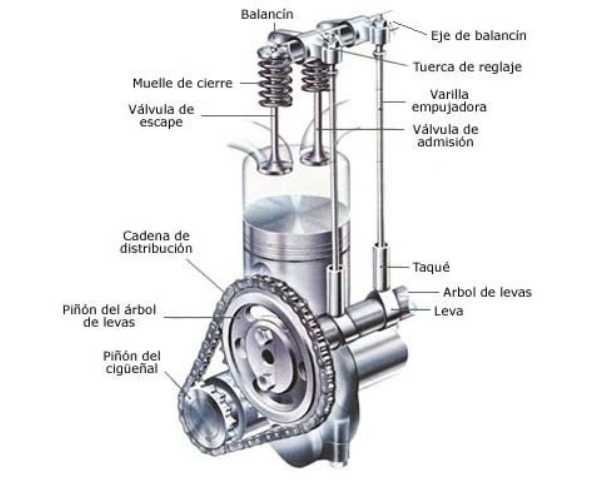
\includegraphics[width=0.5\linewidth]{Figures/01/m2/distrib_schm.jpg}
	\caption{Esquema de un sistema de distribución.}
	\label{fig:dist_schm}
\end{figure}


\subsection{Válvulas} \label{ss:valves}

En un sistema de distribución de un motor alternativo quienes permiten la entrada y salida de los gases, aire y combustible, son las válvulas de admisión y escape. Por ello, se va a analizar cada una de estas válvulas y las principales diferencias que hay entre ellas.\\

La válvula de admisión permite la entrada de aire y combustible en la cámara de combustión. Esta se abre al inicio del proceso de admisión y se cierra antes del proceso de compresión. En general, su tamaño es mayor que las válvulas de escape, facilitando un mayor flujo de entrada. La principal característica de estas válvulas es el diseño de su base, ya que se diseñan para facilitar la mezcla en la cámara introduciendo por ejemplo un hueco en la base para generar turbulencia en el fluido y mejorar la mezcla. En la imagen \ref{fig:int_val} se aprecia un ejemplo de este tipo de válvulas. En cuanto a su material, se suelen fabricar de acero inoxidable, con menos necesidad de soportar altas temperaturas.\\

Las válvulas de escape, por el contrario, permiten la salida de los gases tras completar todo el ciclo; compresión, combustión y expansión. Se abren cuando a de comenzar el escape de los gases y se cierra antes de comenzar nuevamente el proceso de adición. Estas son más pequeñas porque al tener los gases de la cámara alta presión, salen con mayor eficacia por una apertura más pequeña. Su diseño es más simple que el de las válvulas de admisión, pero los materiales deben resistir mejor las altas temperaturas siendo estas normalmente de aceros al cromo o al níquel.


\begin{figure}[H]
	\centering
	\begin{subfigure}[b]{0.45\textwidth}
		\centering
		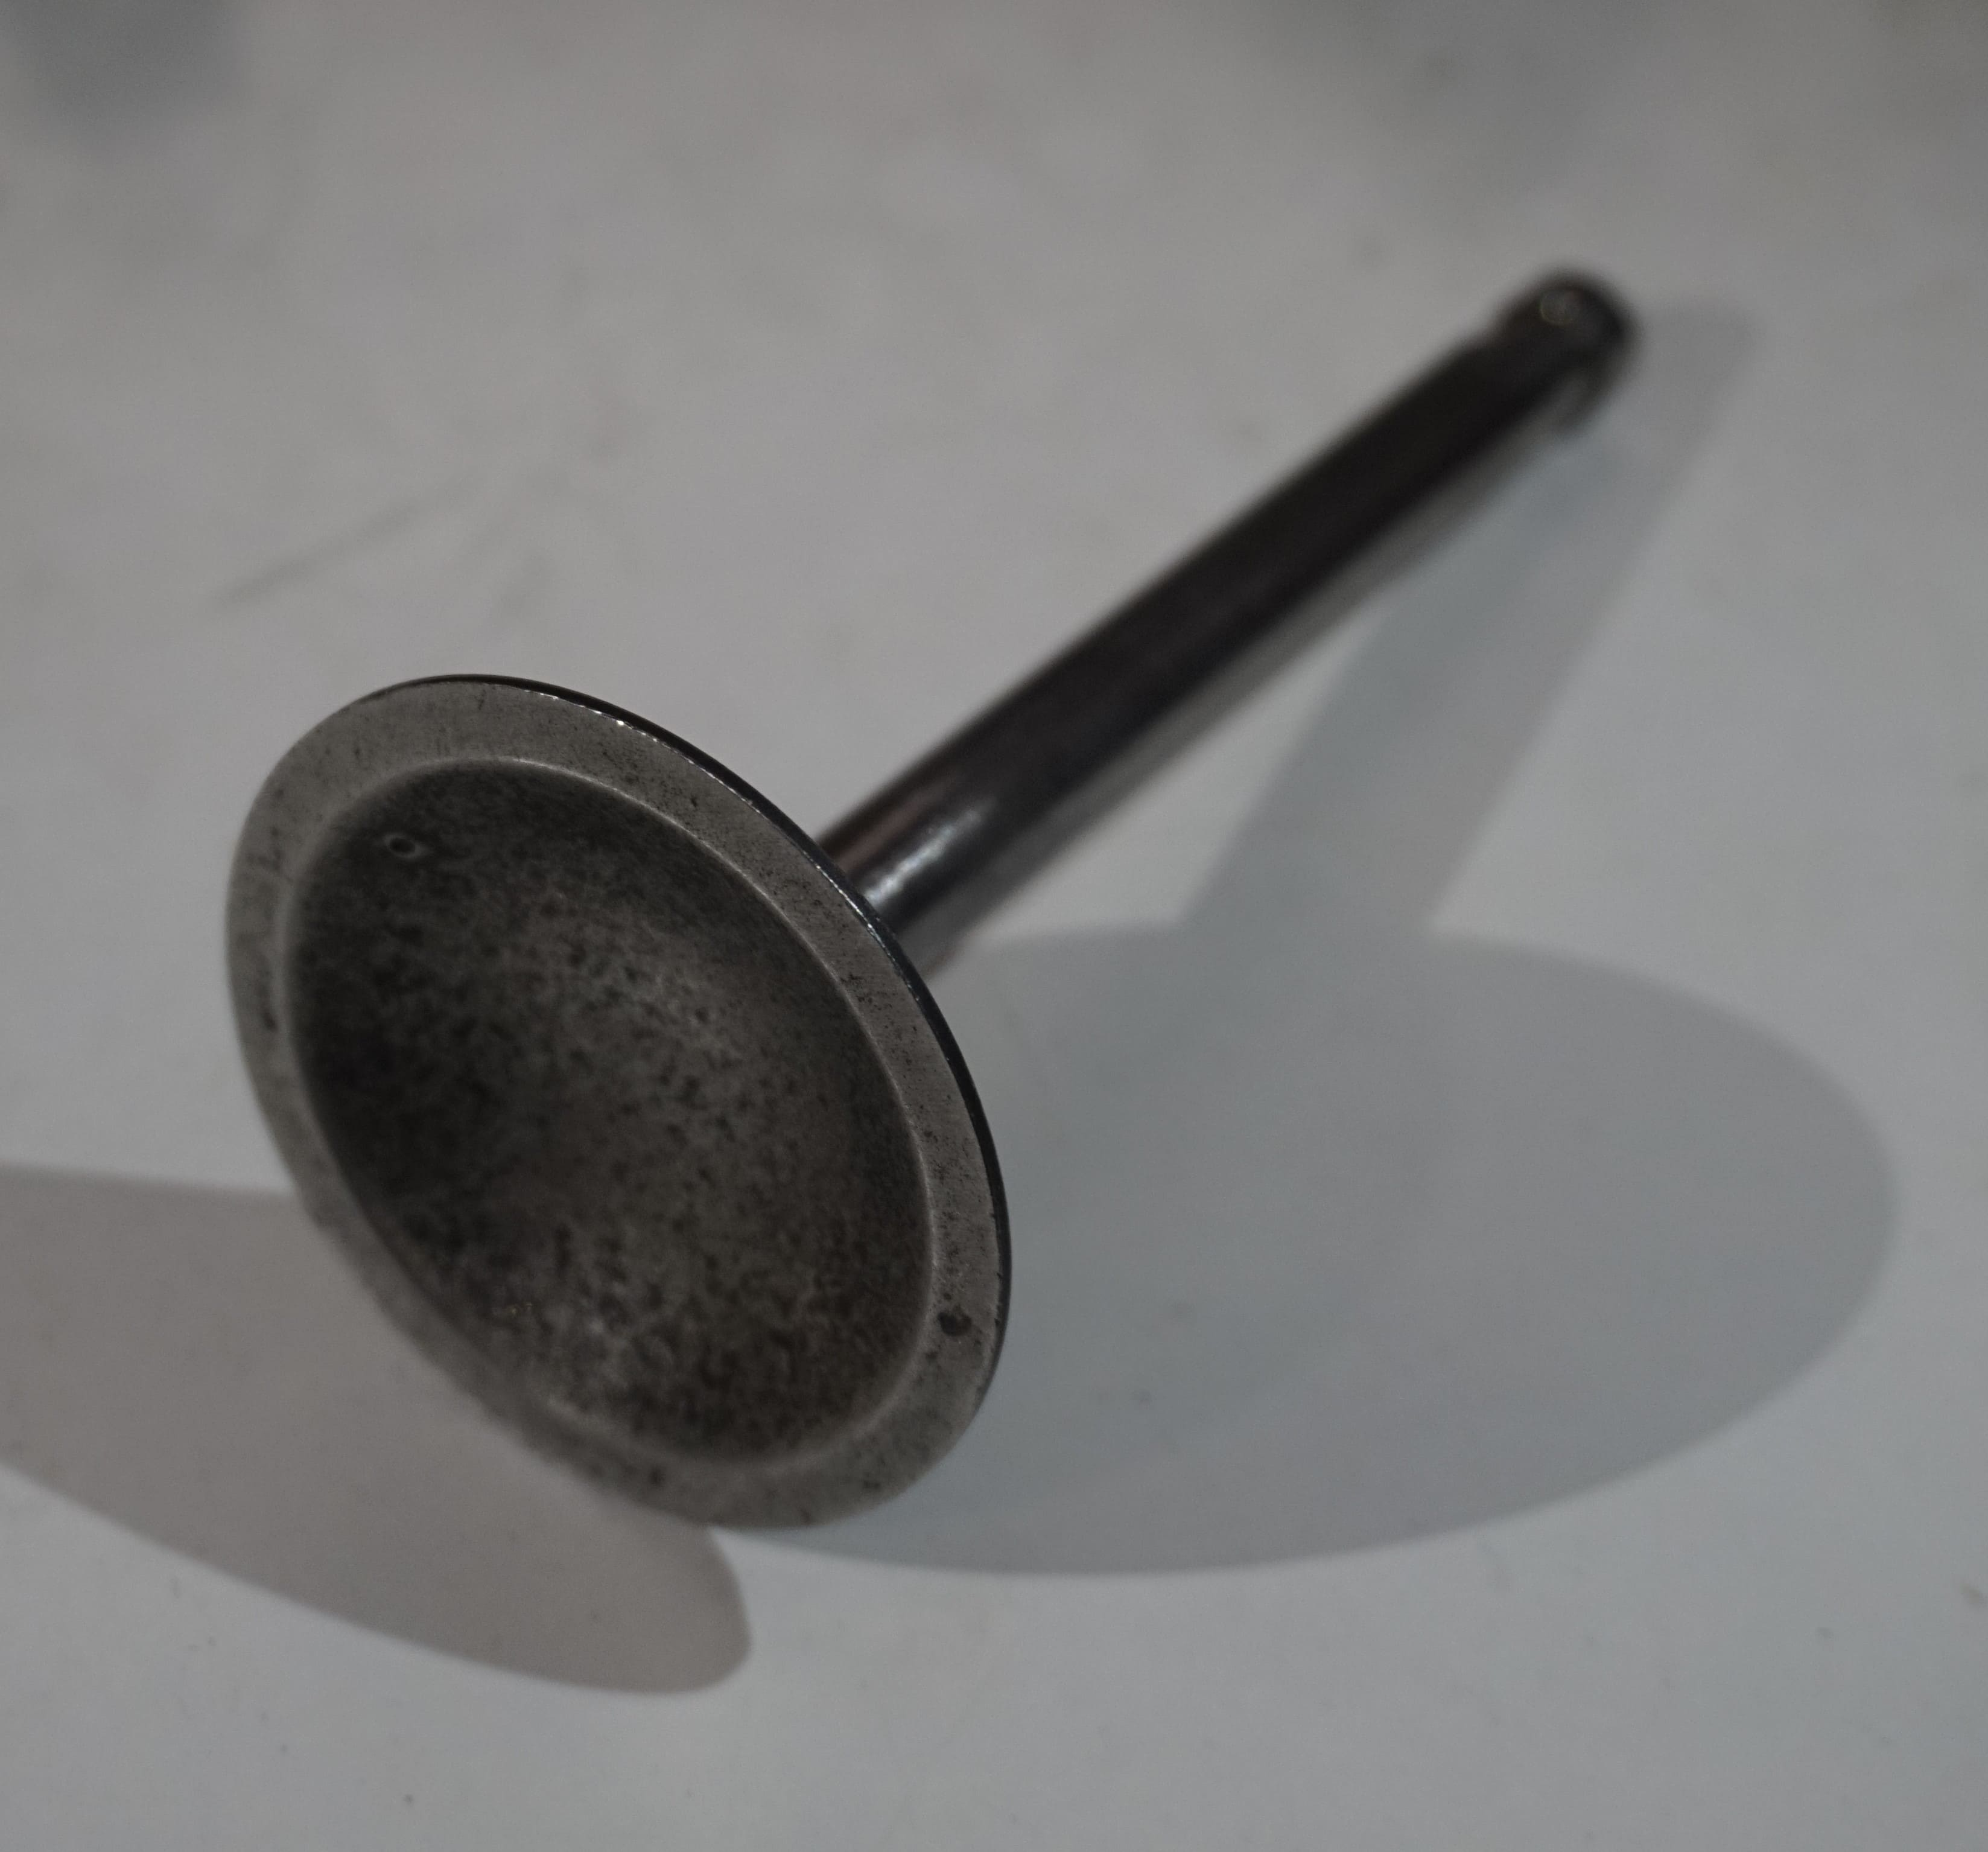
\includegraphics[width=\linewidth]{Figures/01/m2/val_adm.jpg}
		\caption{Válvula de admisión.}
		\label{fig:int_val}
	\end{subfigure}
	\hfill
	\begin{subfigure}[b]{0.45\textwidth}
 		\centering
 		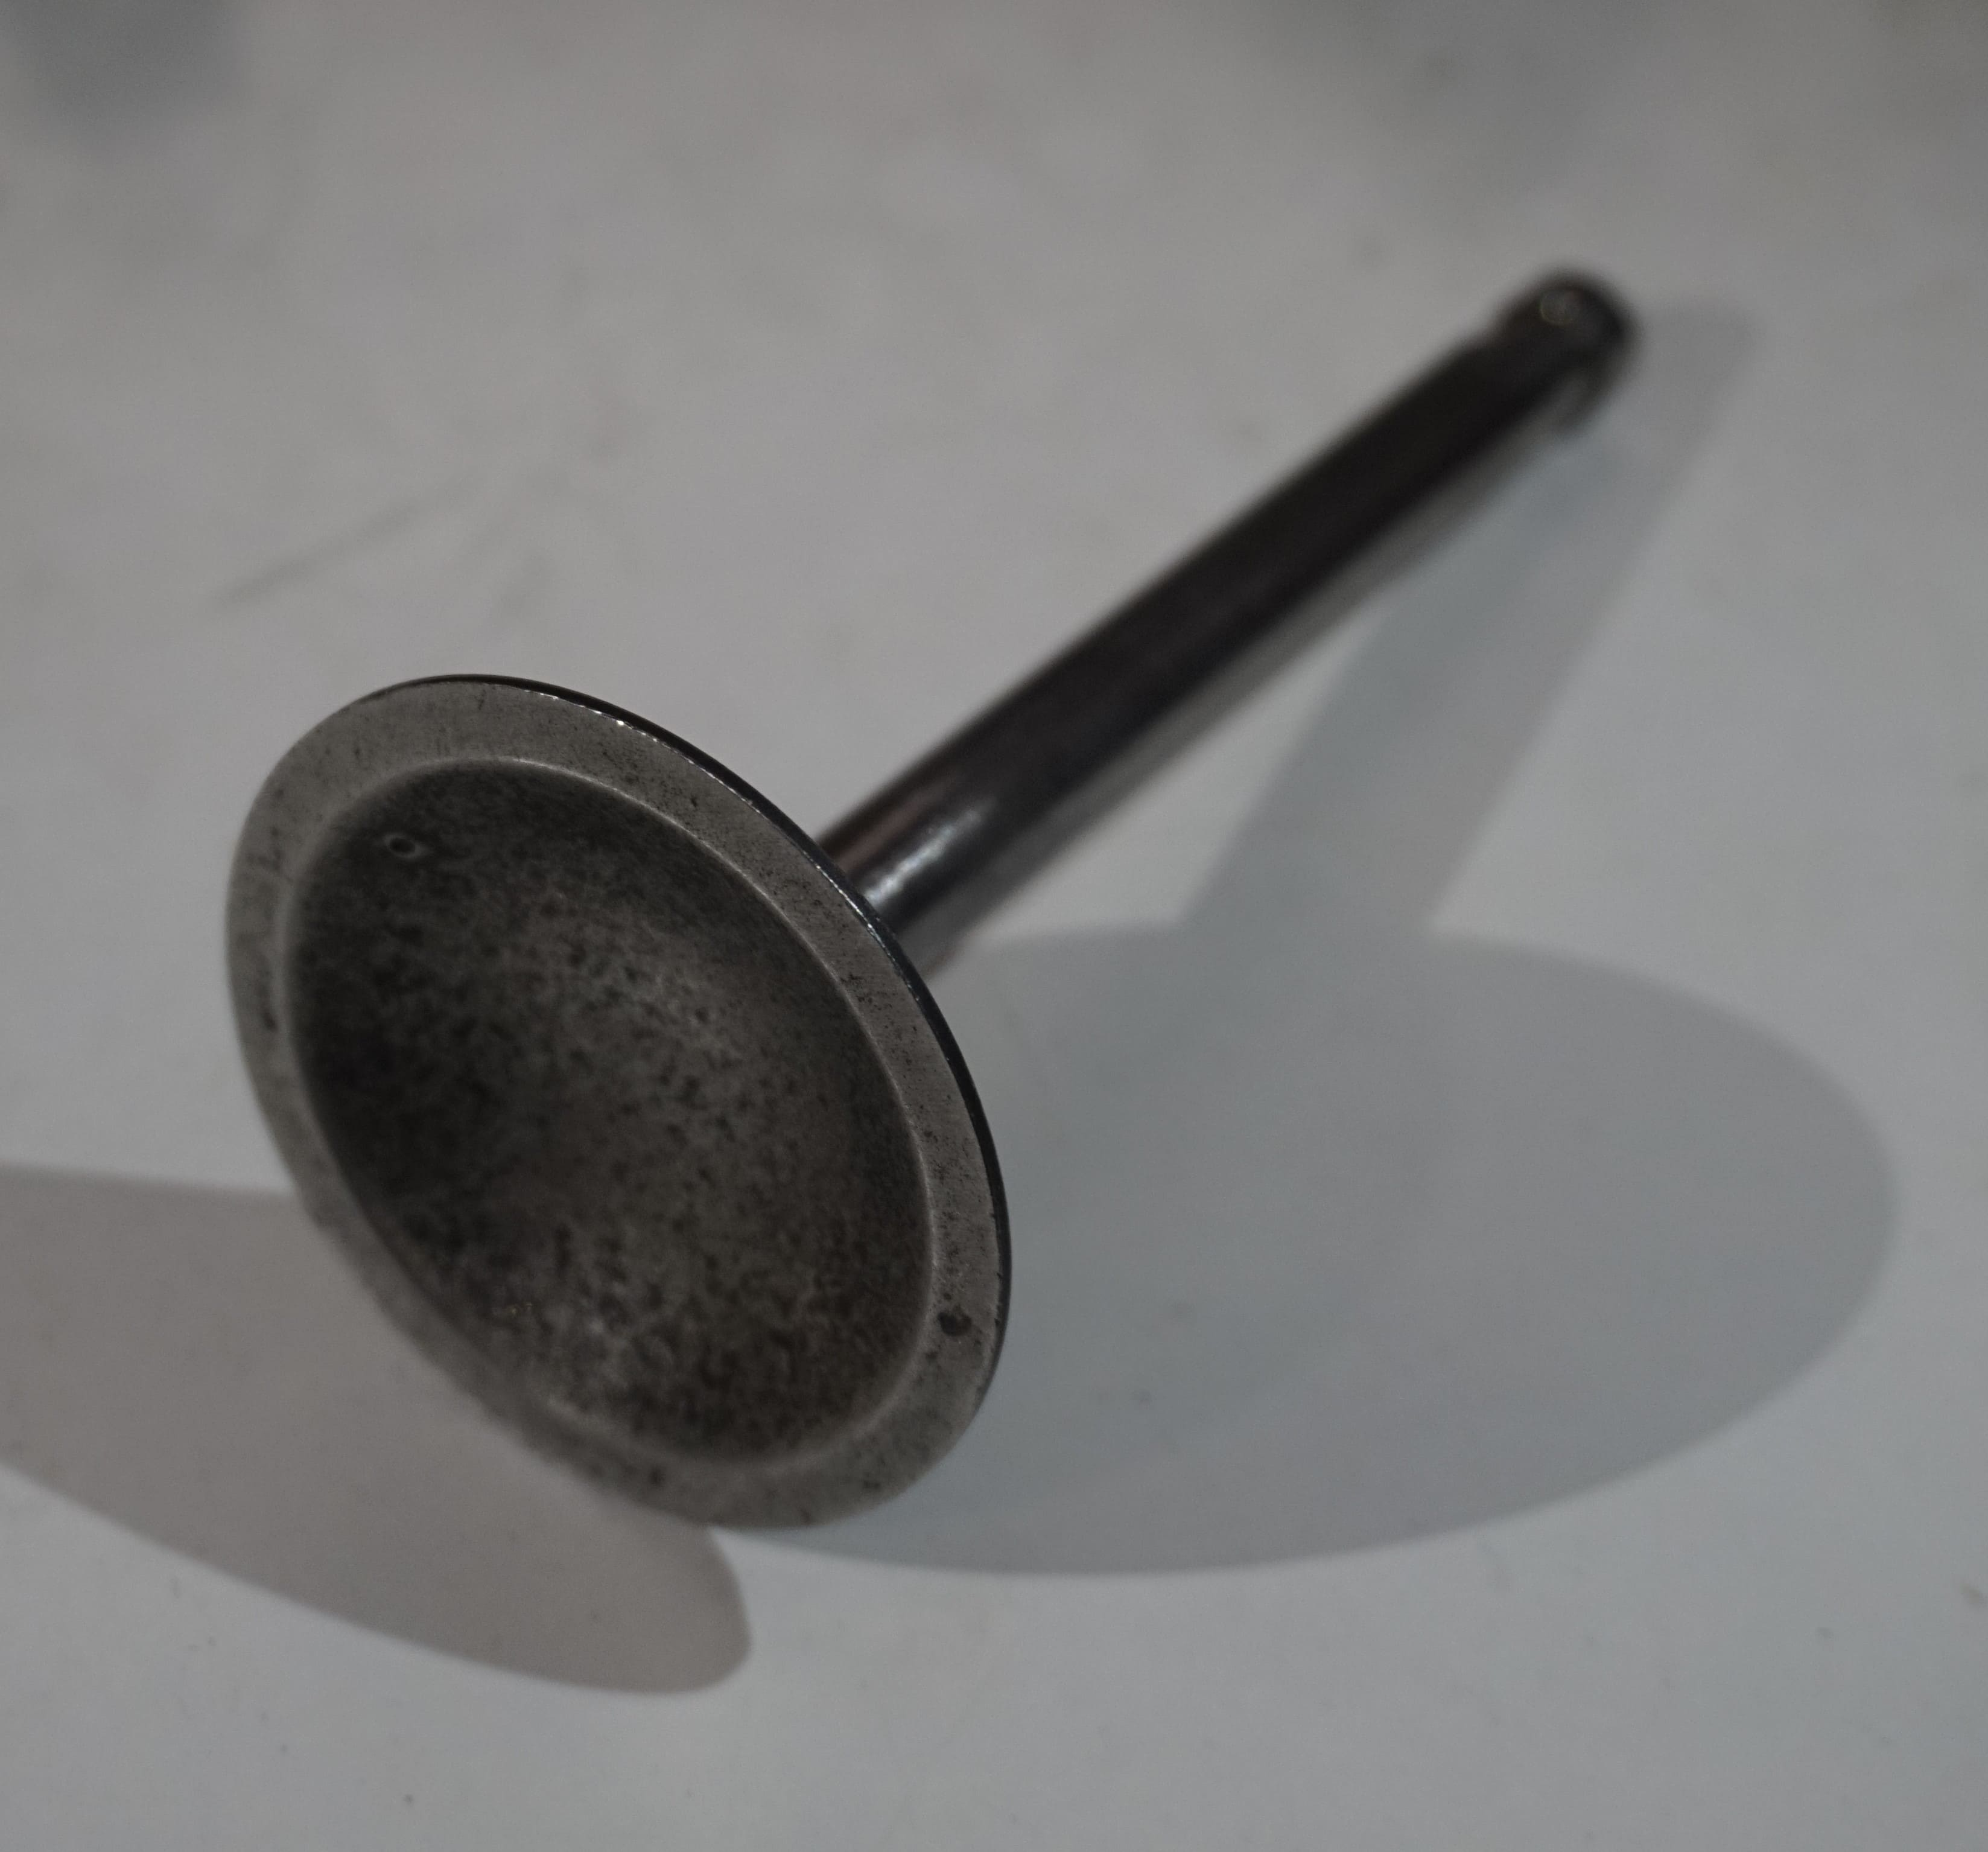
\includegraphics[width=\linewidth]{Figures/01/m2/val_esc.jpg}
 		\caption{Válvula de escape.}
		\label{fig:ex_val}
	\end{subfigure}    
	\caption{Válvulas.}
	\label{fig:valvs}
\end{figure}


En conclusión, la principal diferencia entre una válvula de admisión y otra de escape es su diseño, ya que las de admisión se suelen modificar en su base para favorecer la turbulencia del flujo y mejorar la mezcla en la cámara para obtener un proceso de combustión más óptimo.


\subsection{Árbol de levas} \label{ss:camshaft}

El árbol de levas controla la apertura y cierre de las válvulas de admisión y escape. Mediante protuberancias en el eje empuja los taqués, balancines o directamente las válvulas para permitir el paso de la mezcla aire-combustible y dar salida a los gases de escape.\\

La leva de admisión es generalmente más grande y de mayor duración que la de escape, esto se debe a que esta debe permitir la suficiente cantidad de mezcla, esta leva está optimizada para maximizar la cantidad de aire que entra al cilindro, mejorando así la eficiencia del motor. Por otra parte, las levas de escape son menos pronunciadas, en parte debido a que los gases salen con una presión mayor debida a la combustión.\\

Cabe destacar que en función del motor se pueden encontrar dos árboles de levas, uno de admisión y otro de escape, como se puede observar en la figura \ref{fig:dohc}, o el mismo árbol con ambos tipos de levas.

\begin{figure}[H]
	\centering
	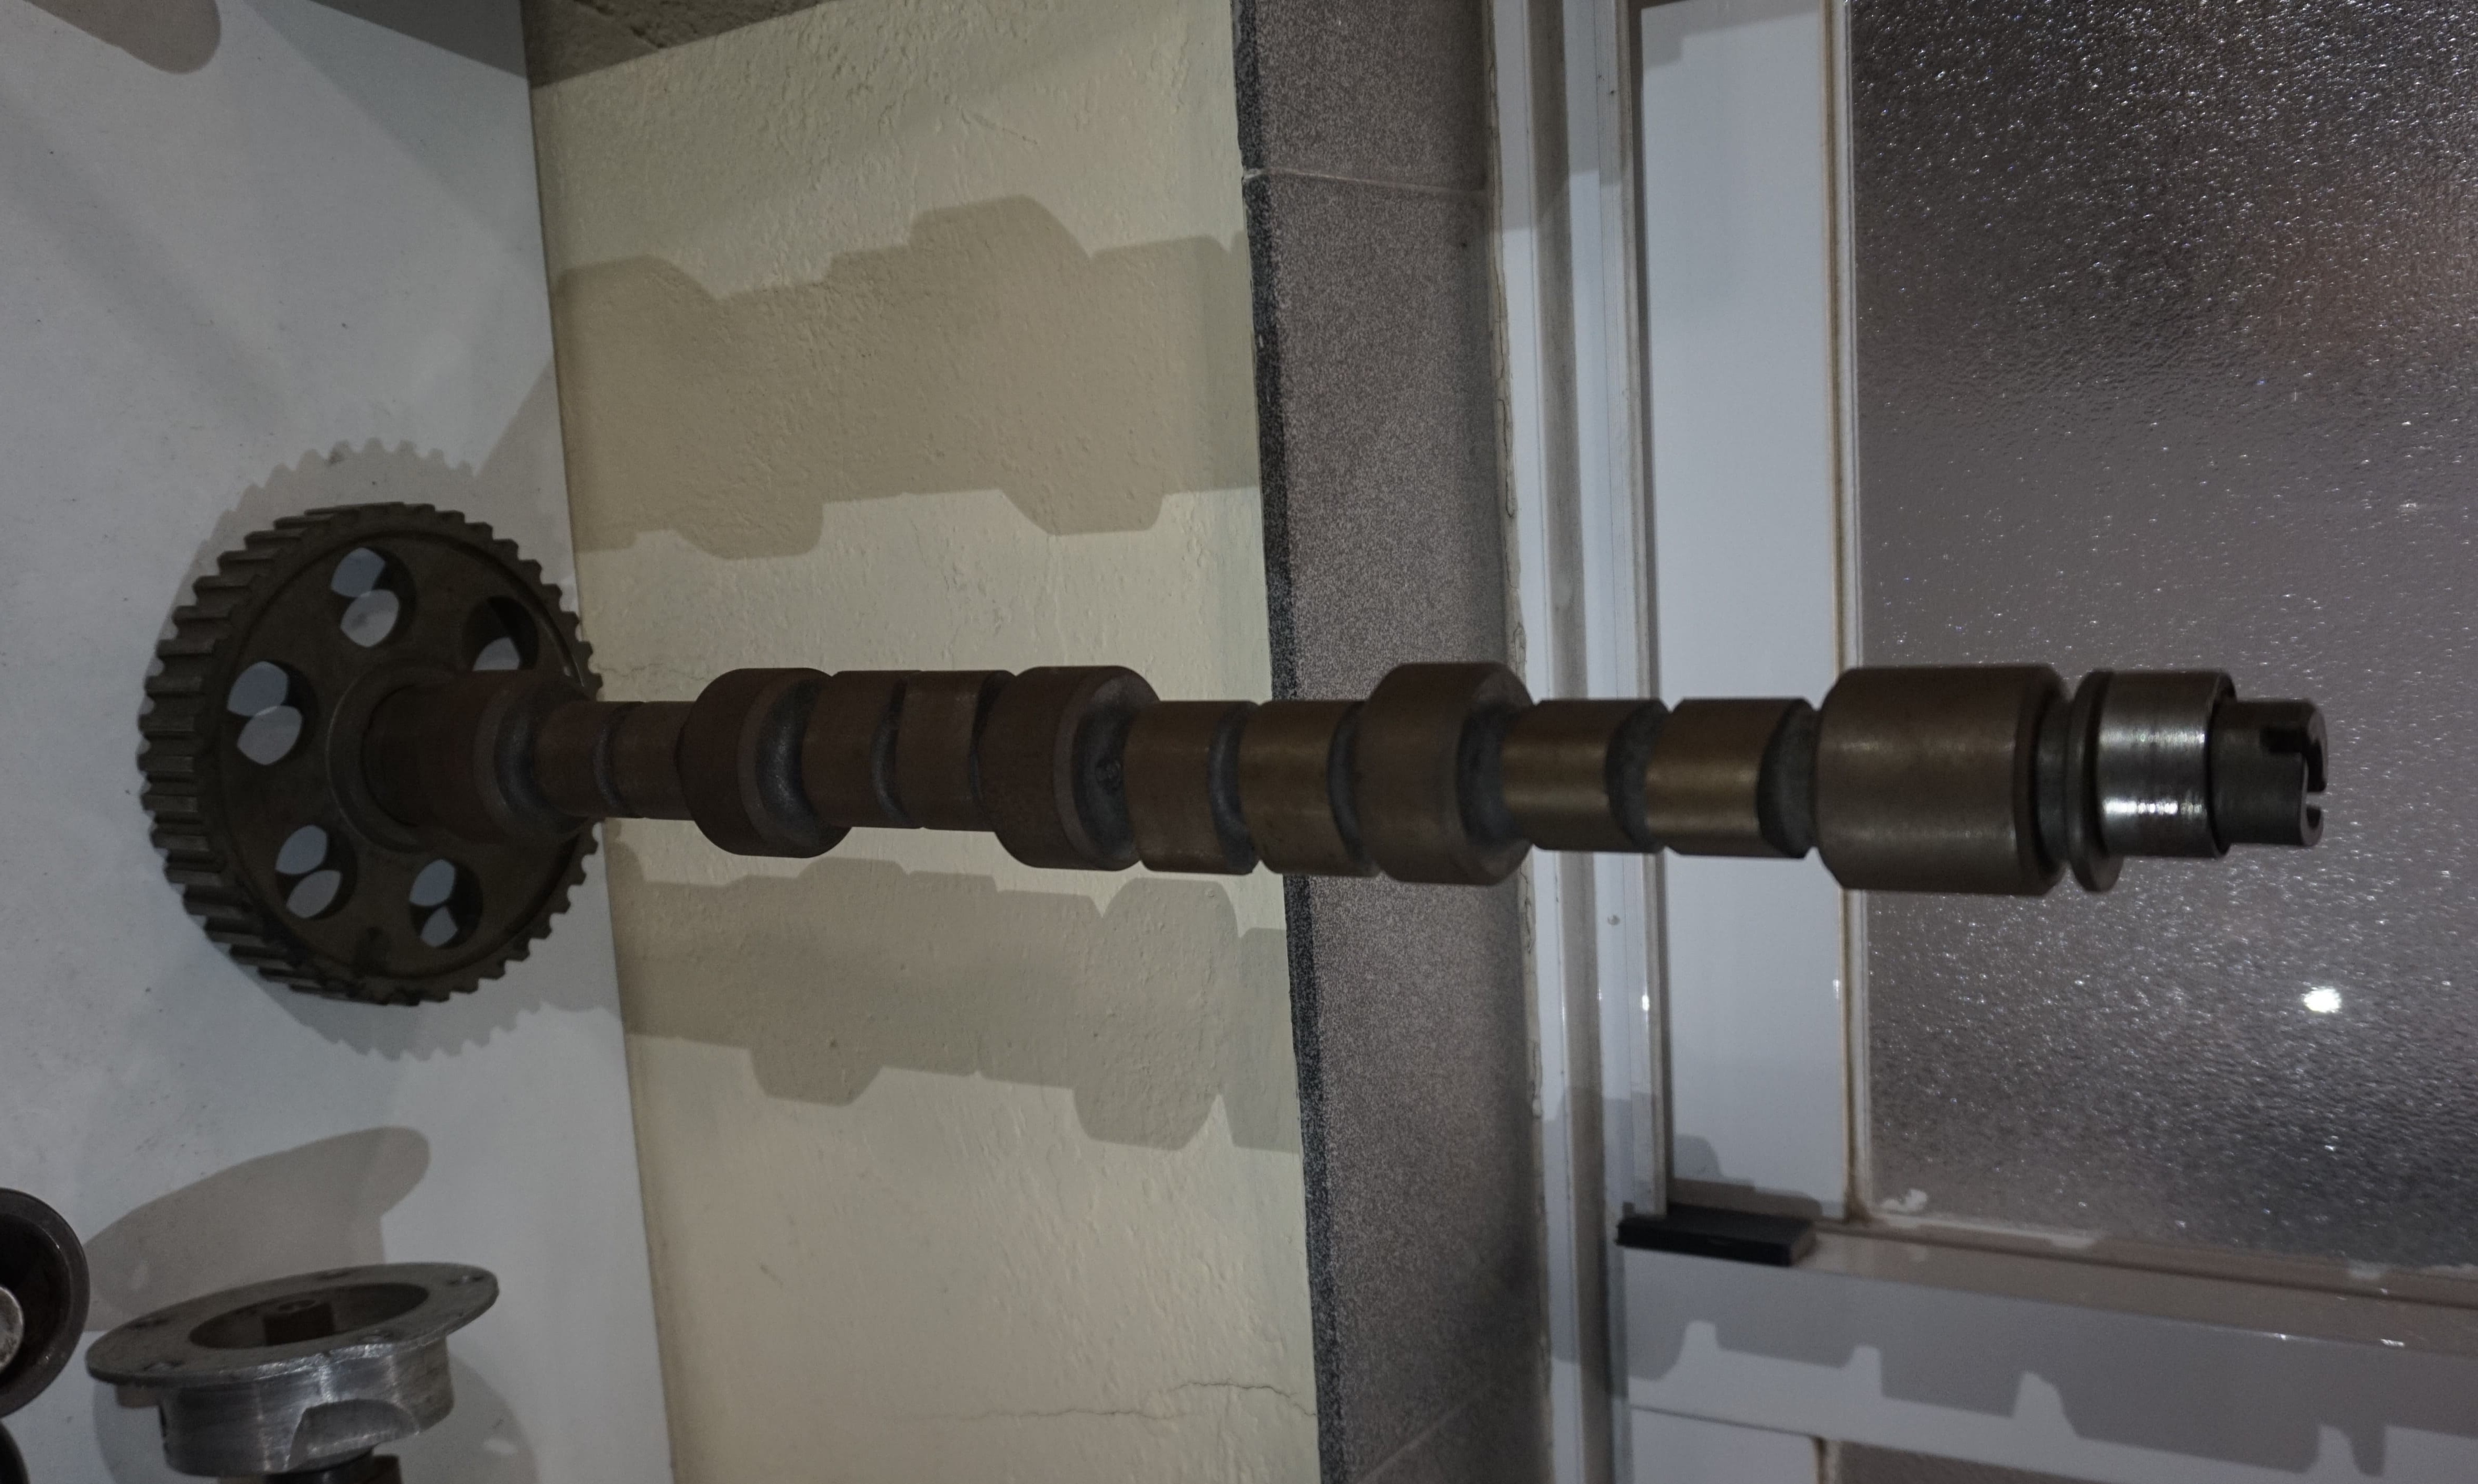
\includegraphics[width=0.6\textwidth]{Figures/01/m2/camshaft.jpg}
	\caption{Árbol de levas.}
	\label{fig:dohc}
\end{figure}

En cuanto a los tipos de configuraciones para los sistemas de distribución, existen varios tipos. En primer lugar están los sistemas de árbol de levas en el bloque, en estos el árbol de levas está ubicado dentro del bloque del motor y acciona las válvulas mediante varillas empujadoras y balancines, tienen una buena durabilidad y un bajo costo, pero tienen limitaciones a altas revoluciones y una mayor inercia. Este sistema se puede observar en la figura 1.\\

Por otra parte están los sistemas de árbol de levas en la culata, en ellos el árbol de levas se ubica en la culata y este acciona las válvulas mediante taqués o balancines cortos. Reducen la inercia de los componentes, por lo que permiten una mejor respuesta a altas revoluciones. Existen dos tipos, los SOHC: poseen un solo árbol de levas en la culata el cual controla tanto las válvulas de admisión como las de escape, y los DOHC los cuales poseen dos árboles de levas, uno para admisión y otro para escape. La figura \ref{fig:DOHC} es un claro ejemplo de un árbol de levas perteneciente a un sistema DOHC.\\

Otro tipo de sistema es el de distribución directa (DOHC sin balancines), en este sistema las levas actúan directamente sobre las válvulas, esto minimiza pérdidas mecánicas y proporciona una respuesta más rápida.

\subsection{Mecanismo de accionamiento del árbol de levas} \label{ss:camshaftchain}

El mecanismo de accionamiento del árbol de levas en los motores alternativos permite que este gire a la mitad de la velocidad del cigüeñal, asegurando que las válvulas se abran y cierren 1 vez en el momento preciso durante los cuatro tiempos del ciclo. Para lograr esto, se utiliza una relación de transmisión 2:1, la cual se implementa generalmente mediante una polea o piñón en el cigüeñal que tiene la mitad del diámetro de la polea o piñón correspondiente al árbol de levas, como se ve en la figura \ref{fig:chain}.

\begin{figure}[H]
	\centering
	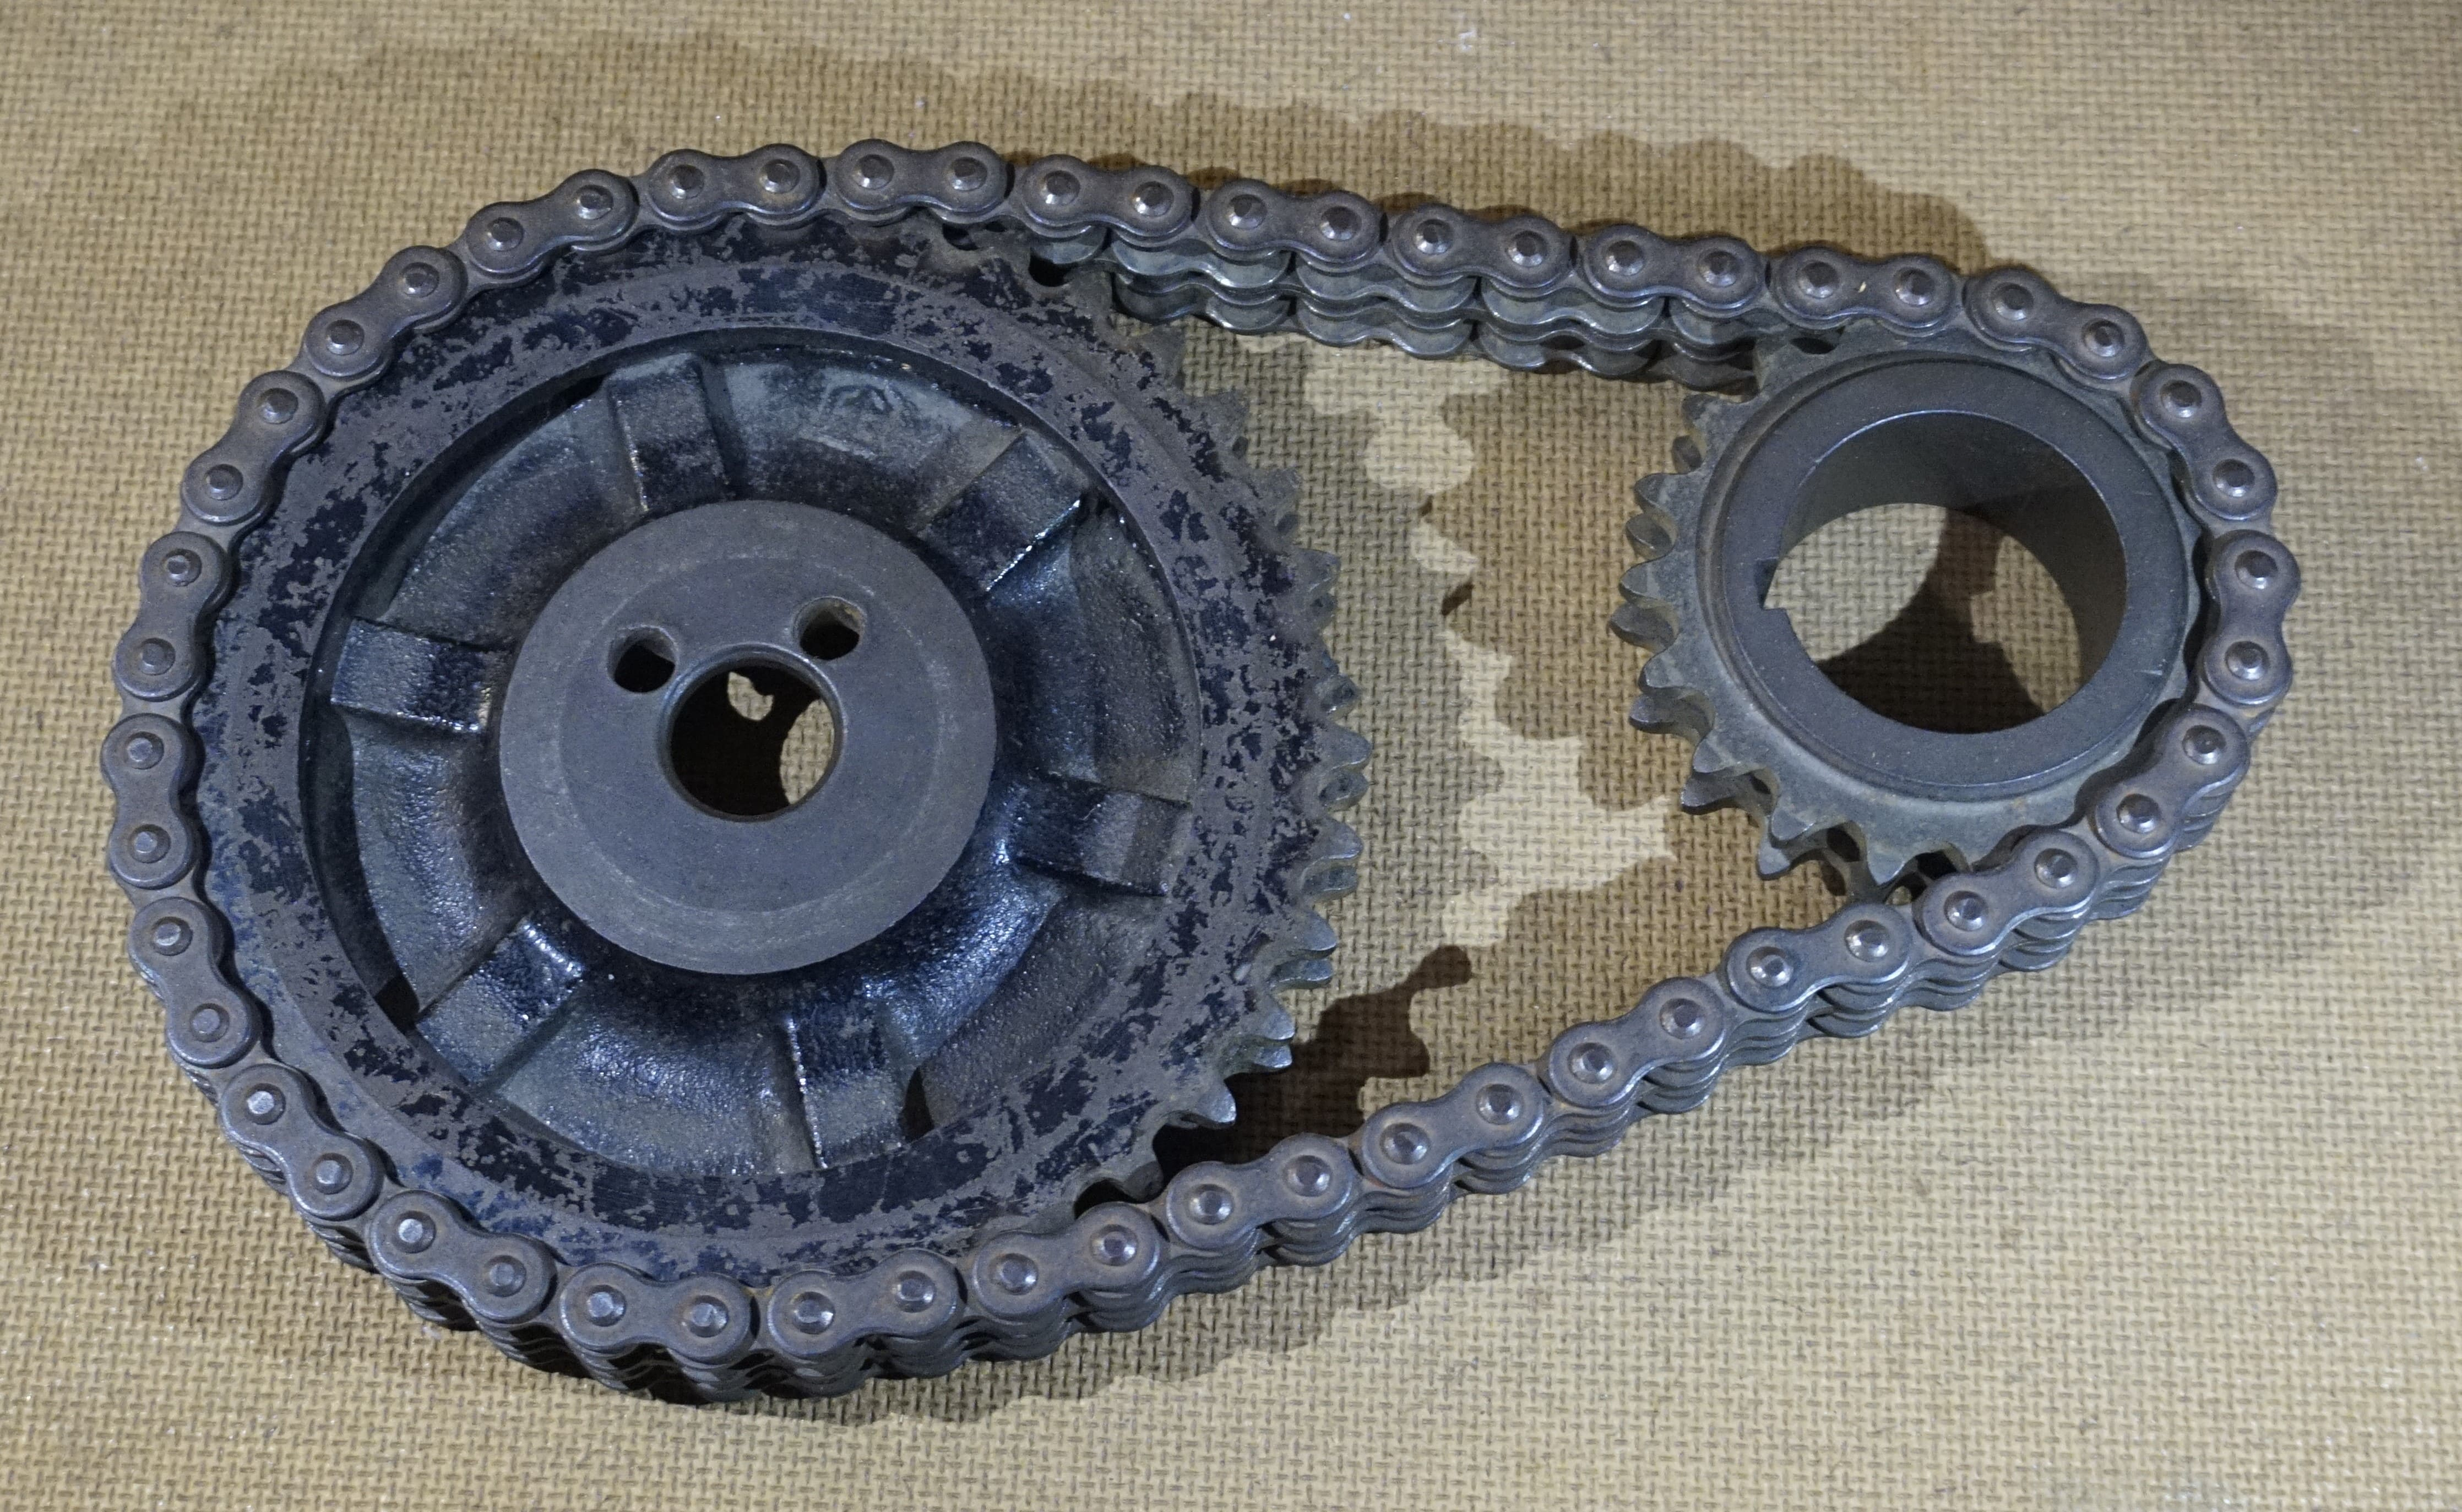
\includegraphics[width=0.6\textwidth]{Figures/01/m2/dist_chain.jpg}
	\caption{Cadena de distribución con sus piñones.}
	\label{fig:chain}
\end{figure}

Existen diferentes medios de transmisión para este mecanismo. Uno de ellos es la cadena, vista en la figura anterior, que ofrece mayor durabilidad y resistencia, así como un menor riesgo de fallos repentinos. No obstante, este sistema tiene desventajas como un mayor nivel de ruido durante su funcionamiento, la necesidad de un sistema de lubricación, y un peso y costo inicial más elevados en comparación con la correa dentada.

Otro de ellos es la previamente mencionada correa dentada, que tiene como ventajas su funcionamiento silencioso, su peso reducido y la facilidad tanto en el mantenimiento como en el reemplazo. Sin embargo, también presenta inconvenientes, como su vida útil limitada debido al desgaste y la posibilidad de rotura, además de su vulnerabilidad a contaminantes como el aceite o la suciedad.

\begin{figure}[H]
	\centering
	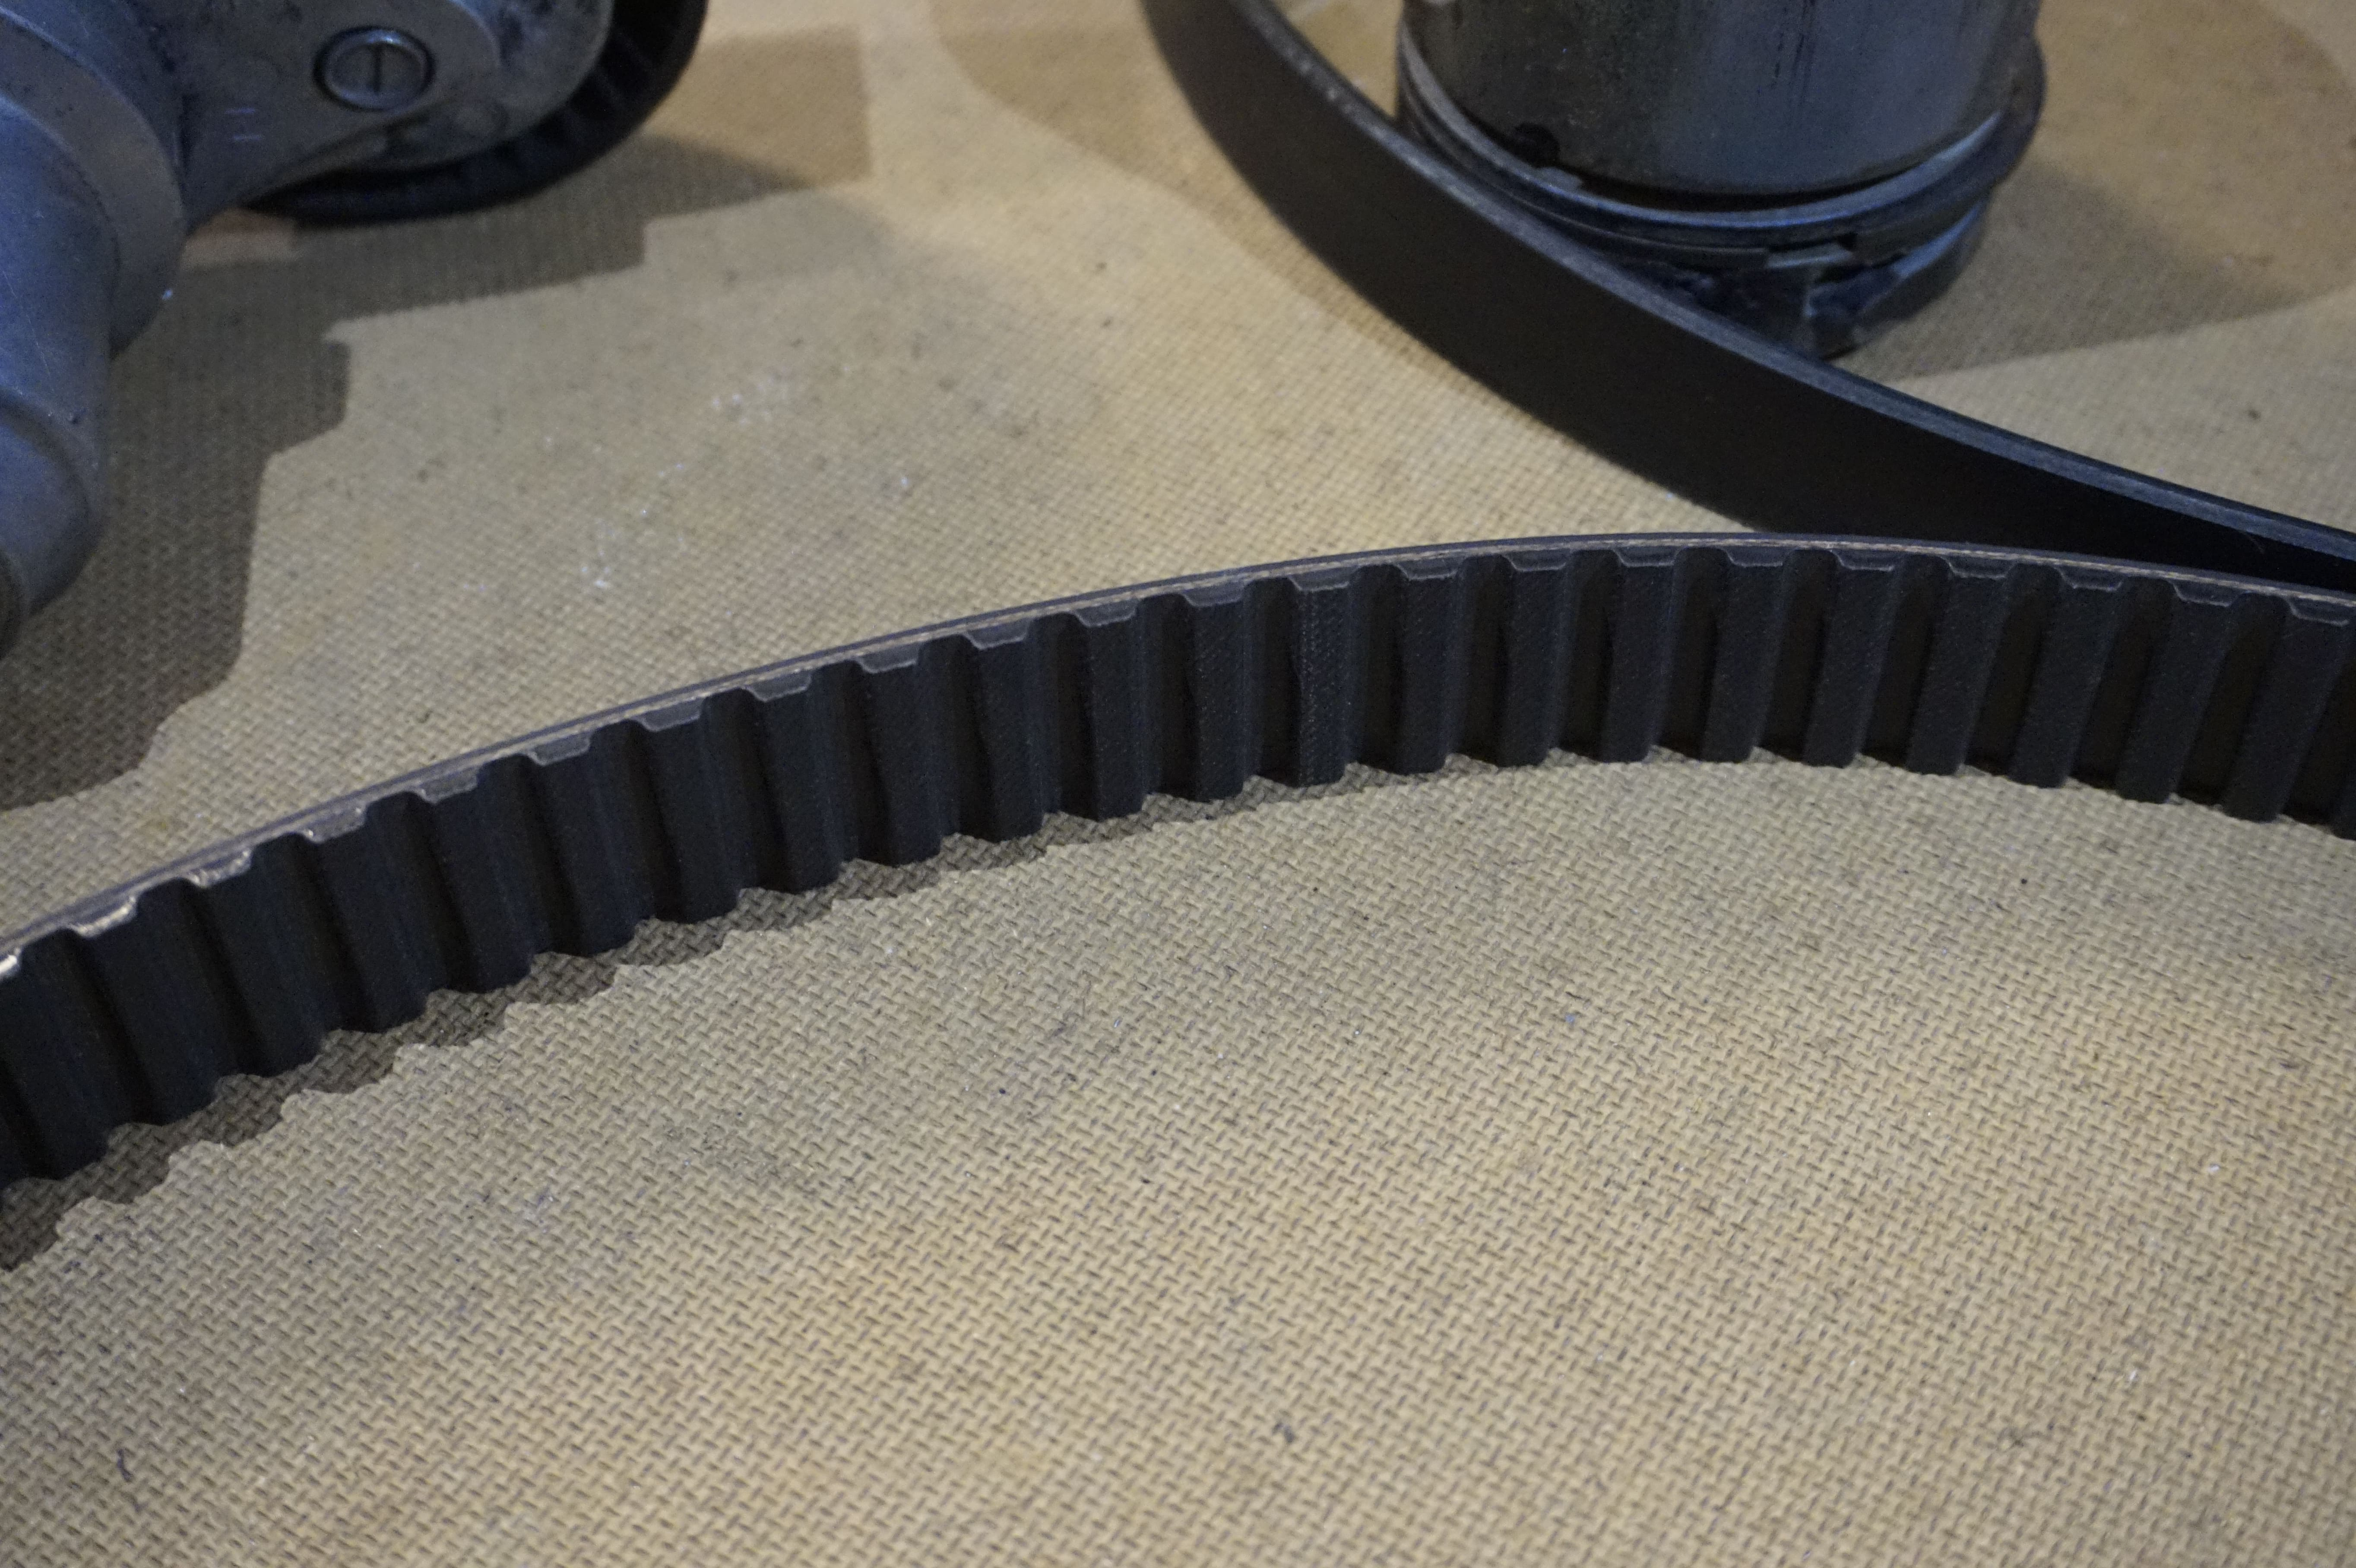
\includegraphics[width=0.6\textwidth]{Figures/01/m2/correa.jpg}
	\caption{Correa dentada.}
	\label{fig:dist_belt}
\end{figure}

La selección entre ambos sistemas depende de las necesidades específicas de diseño, así como de los costos y la durabilidad requeridos para el motor.

\subsection{Levas} \label{ss:cams}

Las levas son los componentes esenciales del árbol de levas, encargadas de transmitir el movimiento a las válvulas para que se abran y cierren en los momentos adecuados. Gracias a la geometría de las levas, cuando el árbol de levas gira las levas empujan el taqué para elevar la varilla empujadora, mover el correspondiente balancín y abrir la válvula.\\

Por este motivo se observa la importancia de que la superficie de las levas sea lo suficientemente dura para soportar la continua fricción con otros componentes del motor. En el caso de no ser lo suficientemente duras se desgastan muy rápido, perdiendo su geometría y no cumpliendo su función, por lo tanto, disminuiría la eficiencia del motor al no permitir la correcta apertura de las distintas válvulas. En la figura \ref{fig:cams} se compara una leva nueva, con otra desgastada por la insuficiencia de dureza superficial.

\begin{figure}[H]
	\centering
	\begin{subfigure}[b]{0.45\textwidth}
		\centering
		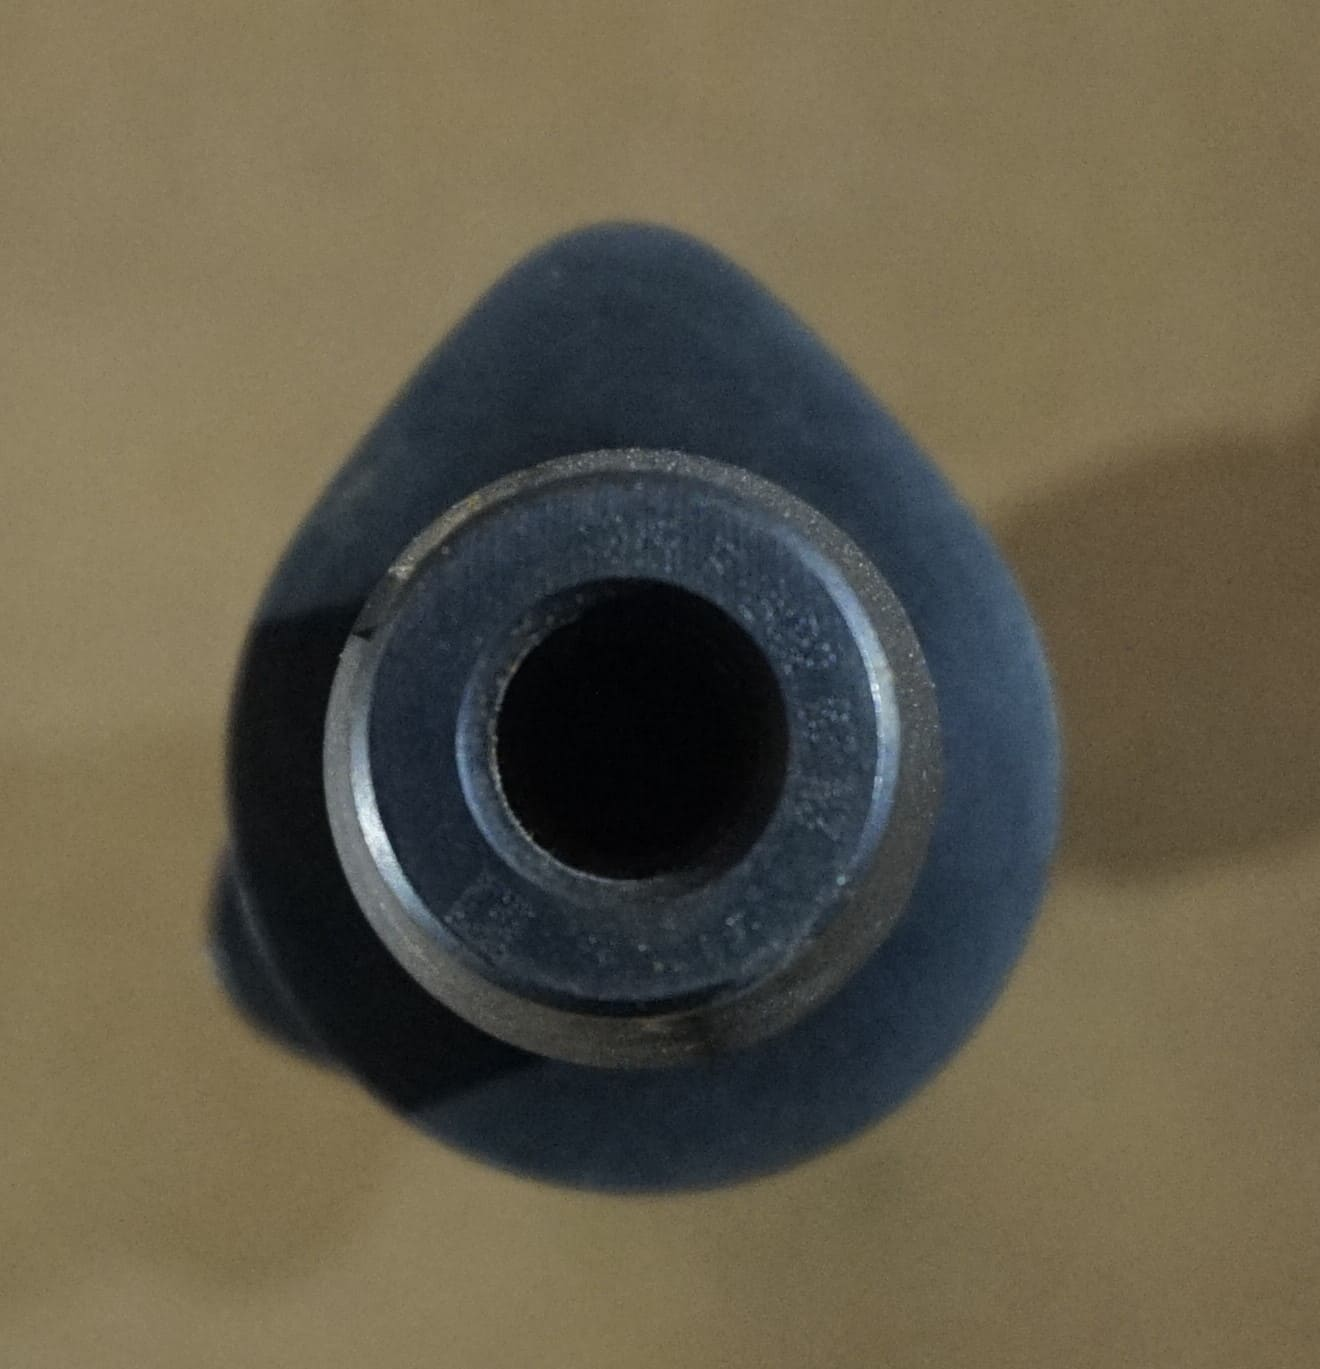
\includegraphics[width=\linewidth]{Figures/01/m2/leva_nueva.jpg}
		\caption{Leva en correcto estado.}
		\label{fig:new_cam}
	\end{subfigure}
	\hfill
	\begin{subfigure}[b]{0.45\textwidth}
 		\centering
 		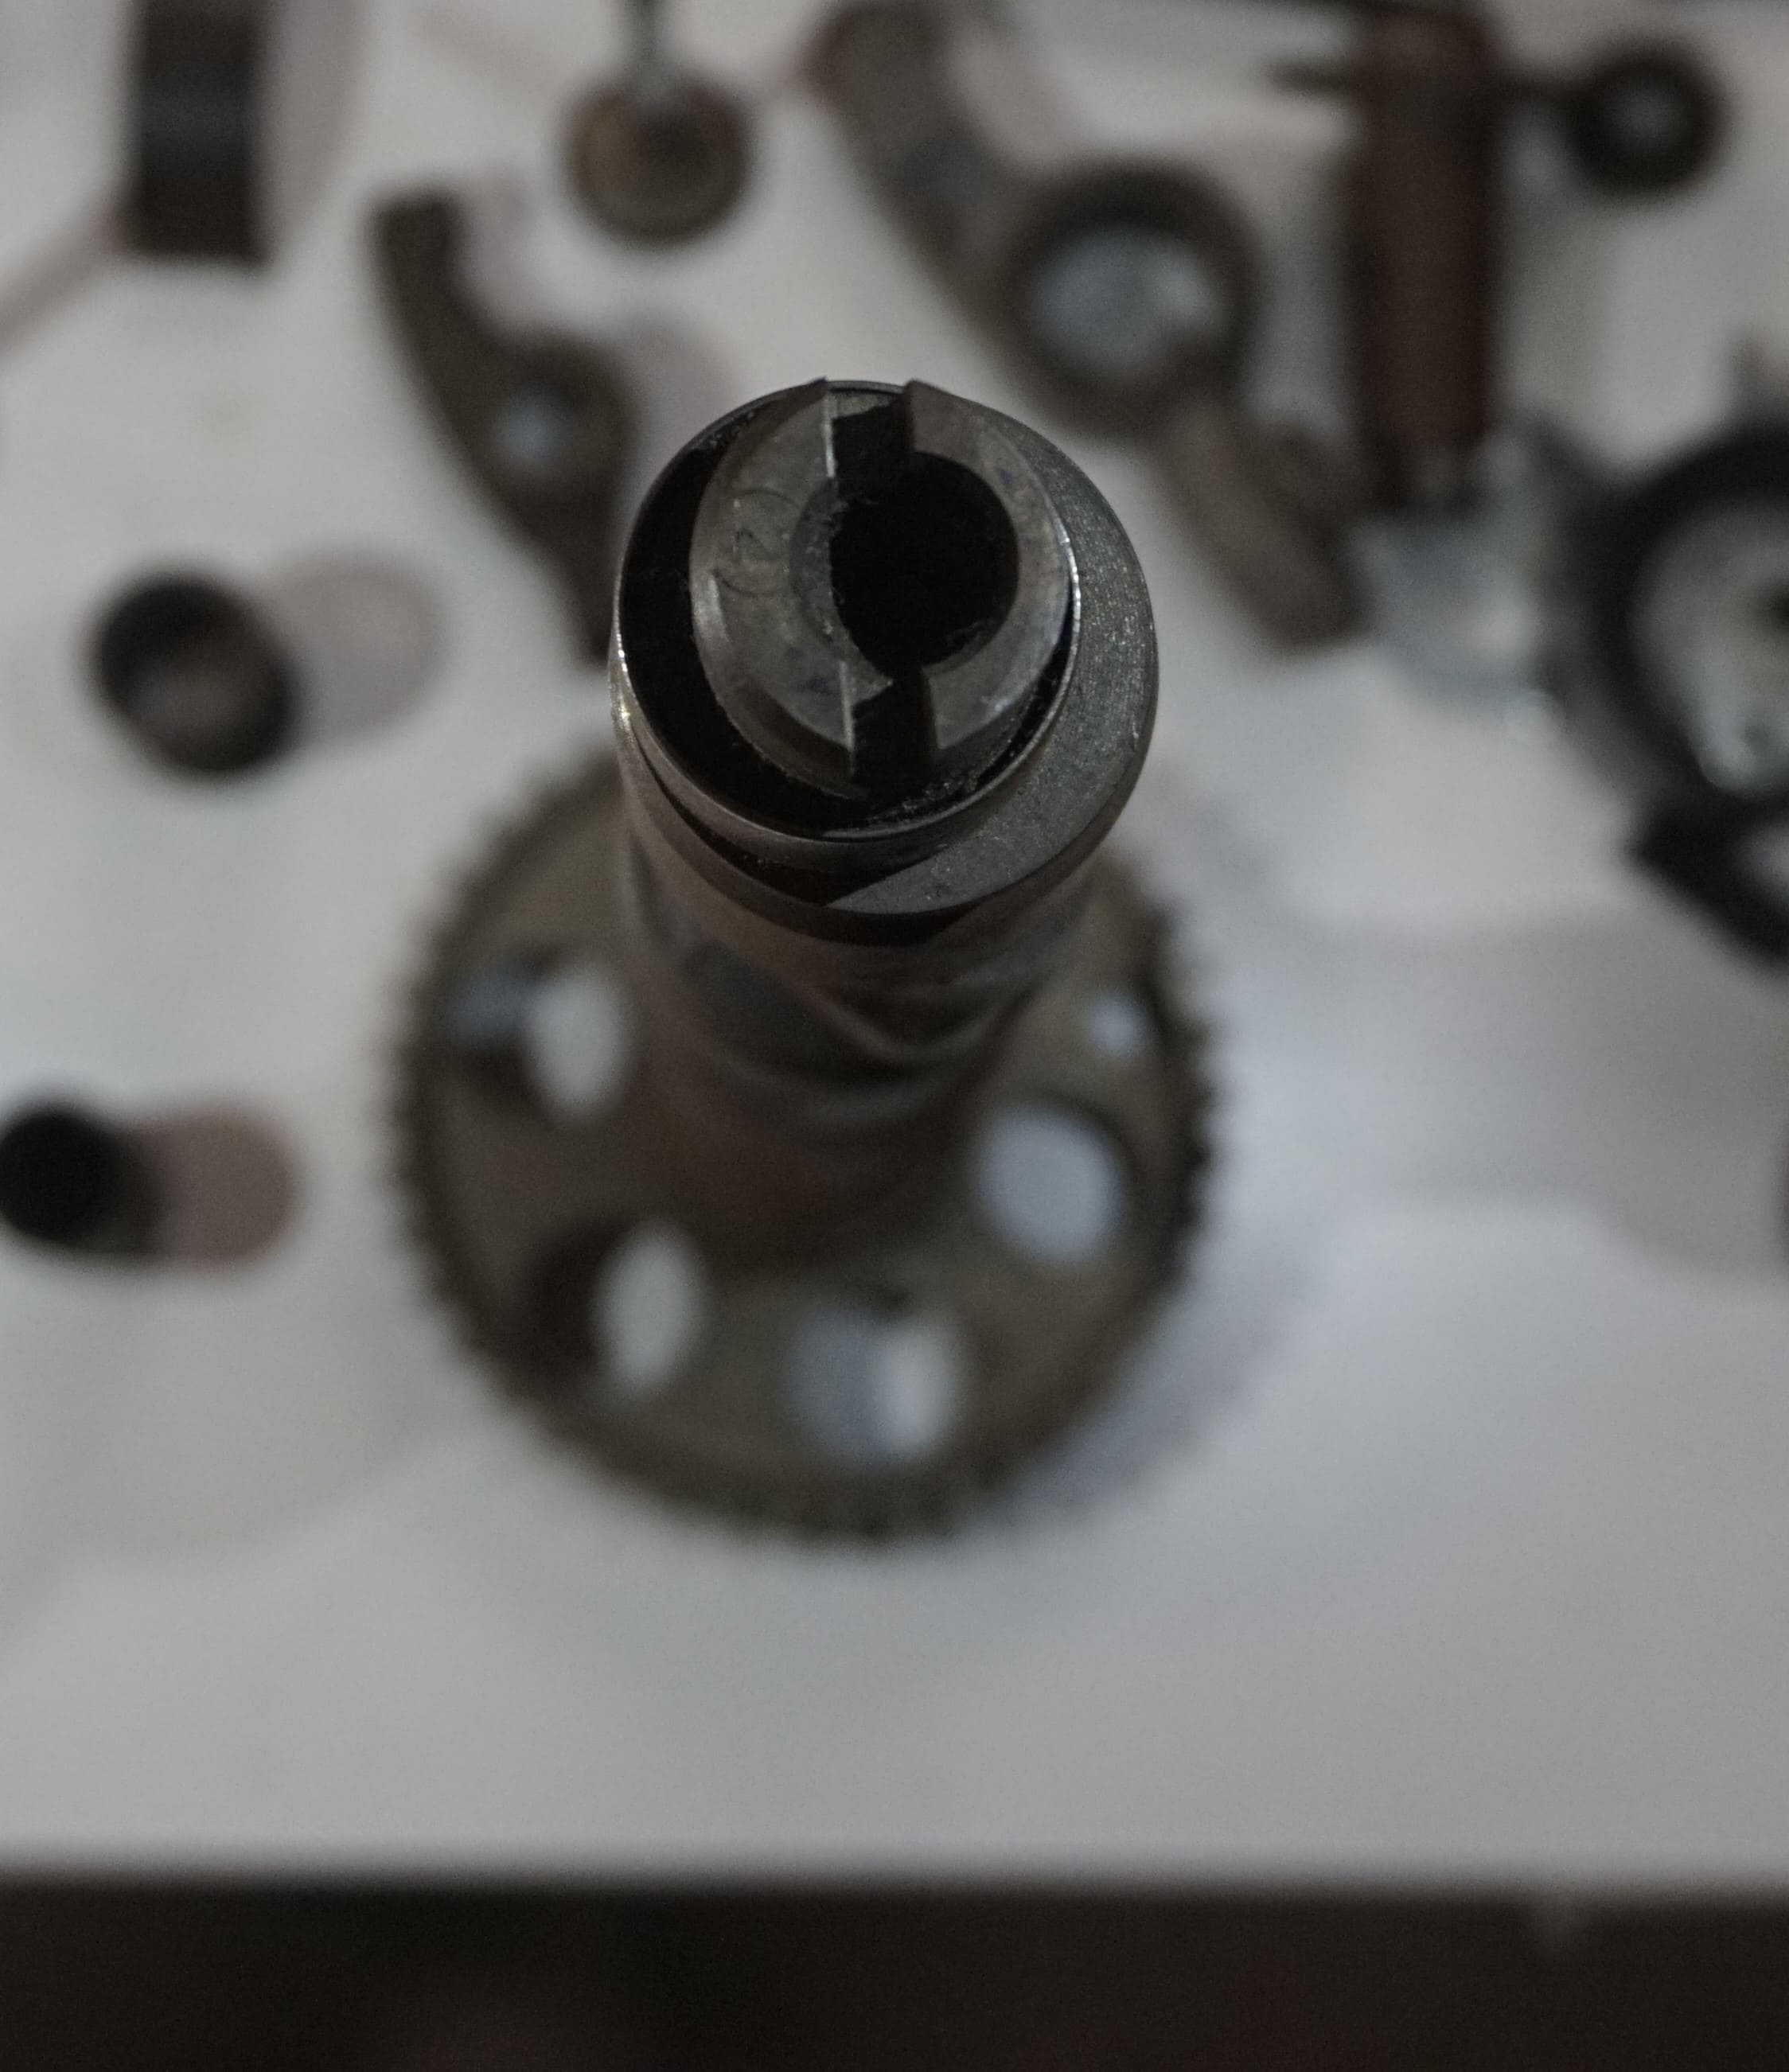
\includegraphics[width=\linewidth]{Figures/01/m2/leva_desgastada.jpg}
 		\caption{Leva con pérdida de perfil.}
		\label{fig:brk_cam}
	\end{subfigure}    
	\caption{Levas en distintos estados de conservación.}
	\label{fig:cams}
\end{figure}

Por ello a las levas se les da tratamientos de endurecimiento superficial. En cuanto al núcleo las levas son más blandas buscando resistencia al impacto y la prevención de fracturas. Debido a la combinación de durezas en la leva se consigue que estas soporten las cargas dinámicas sin fallar.
